\chapter{网侧先进绝热压缩空气储能电站建模及运行方法}
\label{cha:aa-caes}

\section{概述}
\label{sec:aa-caes-intro}
~AA-CAES~在新能源电力系统中最基本的应用形式即为储能电站,可用于电网削峰填谷、调峰、备用等场景。AA-CAES能用于该类场景的主要原因在于其能为电网提供较长时间的能量及容量备用等灵活性支撑(见图\ref{fig:CAES-AS-Overview}),而实现~AA-CAES~储能电站能量与备用特性的准确建模是分析其在电力系统中运行特性的前提。

构建能量与备用模型最直观的思路是采用等效电池模型,然而本文第\ref{cha:simulation}章指出备用等运行模式需要AA-CAES储能电站运行于宽工况条件,导致内部组件处于部分负载运行模式,而等效电池模型难以刻画组件级的部分负载特性。另一方面,完全采用第\ref{cha:simulation}章的部分负载热力学仿真模型构建的能量与备用模型又过于复杂,难以被实际AA-CAES储能电站及所在电力系统的运行调度所采用。为此,我们需要寻求一种既不丢失AA-CAES的宽工况热力学特性且物理意义简单明确的运行建模方法,以实现等效电池模型与热力学仿真模型之间的平衡。

借鉴数据结构的思想,若将AA-CAES视为对象,其属性可视为第2章研究的每个组件,而其方法为各组件的部分负载热力学特性。只要通过合适的接口设计,使得AA-CAES这一对象对外提供能表征其内部热力学特性,且对外部应用而言物理意义明确、形式简单的典型接口函数,即可实现复杂的热力学仿真模型与电力等效电池模型间的平衡。本章将该类接口函数称为热力学特性曲线簇,其可实现对内部组件级部分负载特性的封装,同时对外提供了获取AA-CAES系统宽工况运行特性的接口,可供储能电站的调度运行及市场运营等问题使用。

本章结构安排如图~\ref{fig:AA-CAES-Flow-Chart}所示,第~\ref{sec:chap3-aa-caes-sim}节基于第~\ref{cha:simulation} 章组件级部分负载热力学仿真模型,提出表征AA-CAES宽工况运行特性的热力学特性曲线簇;第\ref{sec:dual-SOC}节基于宽工况特性曲线簇,提出计及储气水平与储热水平及二者耦合关系的双~SOC~建模框架与方法;第
\ref{sec:chap3-wind-ESS-operation}节基于双~SOC~模型分析宽工况特性对风-储协同系统运行的影响;第\ref{sec:chap3-bid-aa-caes}节给出AA-CAES储能电站的市场运营策略,以提升储能电站运行经济性。

\begin{figure}[H] % use float package if you want it here
  \centering
  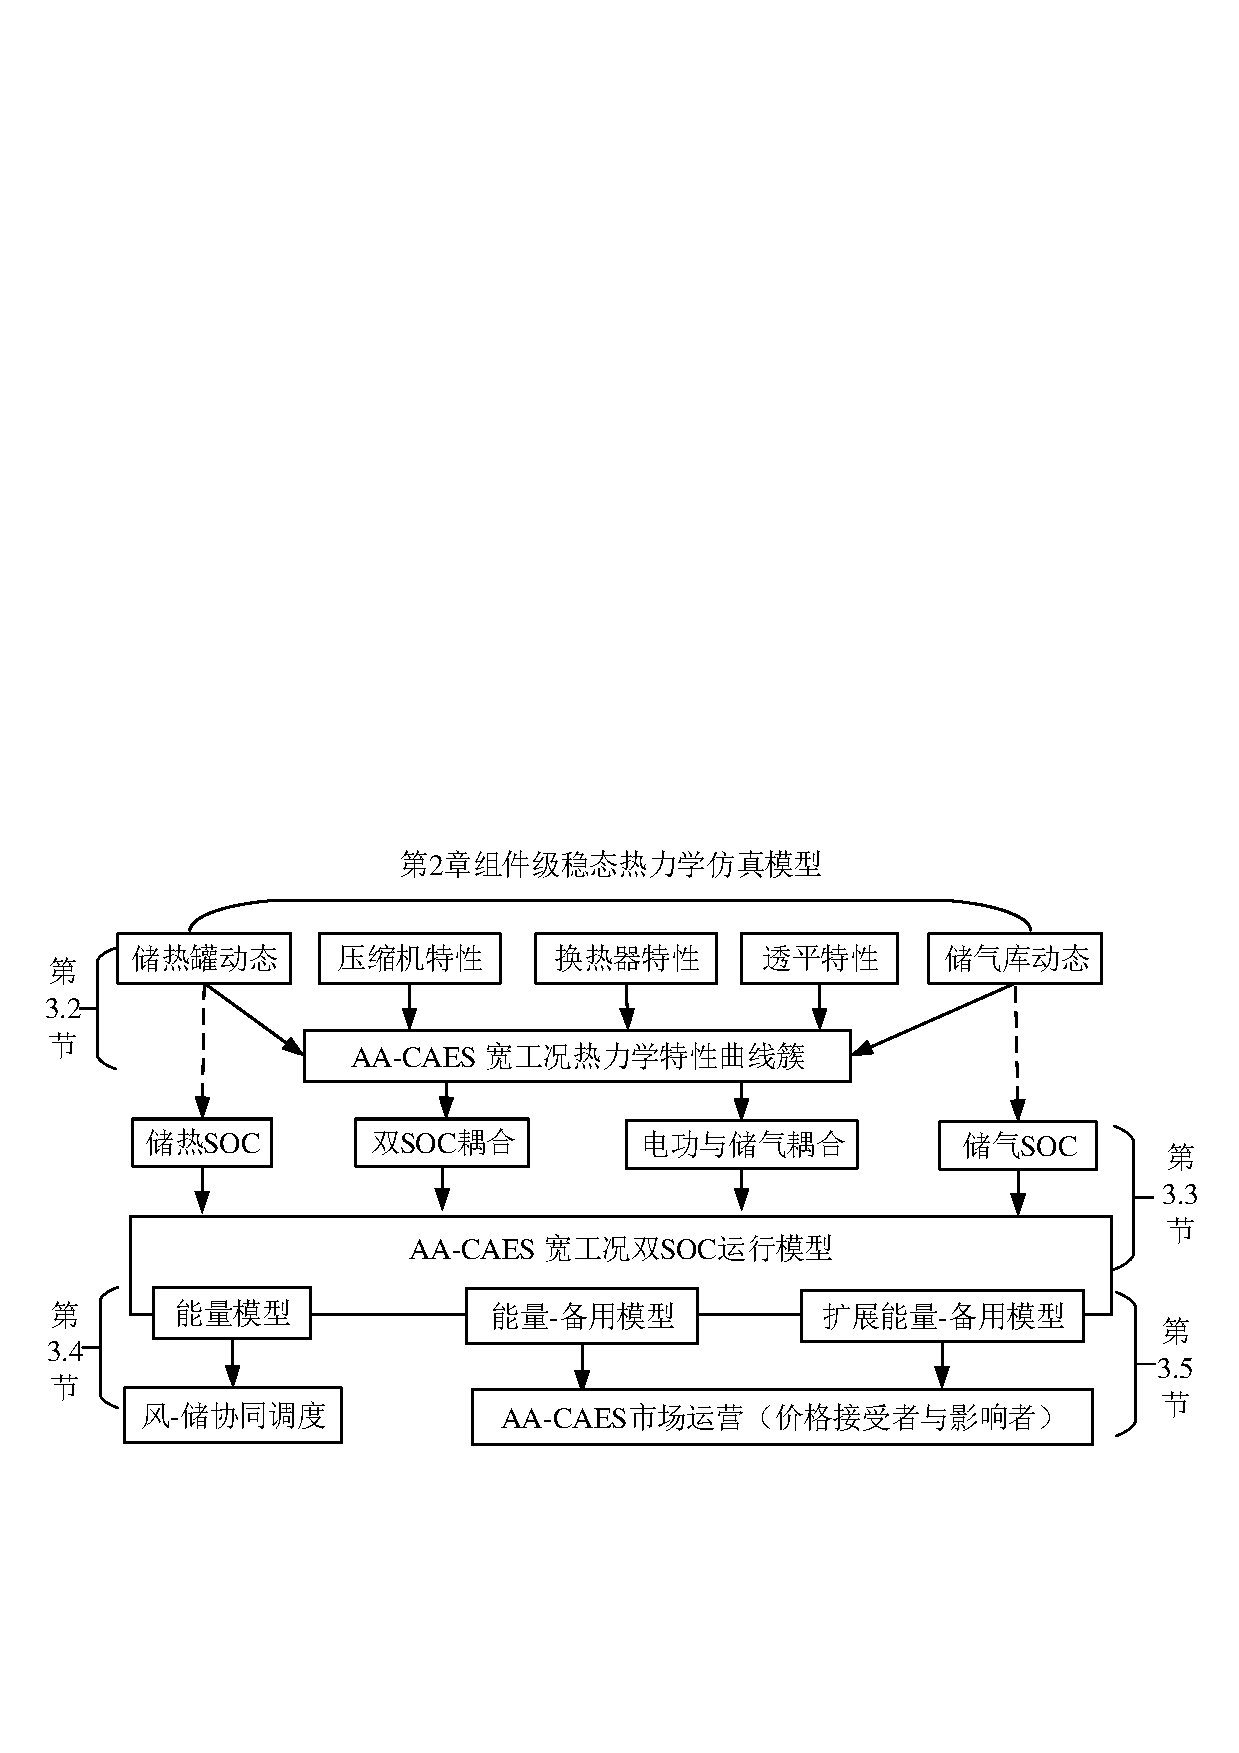
\includegraphics[scale=0.72]{figures/Chap3-1-AA-CAES-Flow-Chart-V4.pdf}
  \caption{第~\ref{cha:aa-caes}~章结构安排}
  \label{fig:AA-CAES-Flow-Chart}
\end{figure}

\section{宽工况热力学特性曲线簇}
\label{sec:chap3-aa-caes-sim}
本节基于第\ref{cha:simulation}章宽工况热力学仿真模型抽象出能刻画AA-CAES内部组件的部分负载特性对系统宽工况运行特性整体影响的热力学特性曲线簇。首先,分析AA-CAES 内部组件级(压缩机、膨胀机、换热器)部分负载特性的集中化表示思路;其次,从换热器视角给出AA-CAES内部压力势能与压缩热能双能流耦合关系的集中模型;最后,从压缩机与膨胀机视角给出储气量与压缩/膨胀功率间的耦合关系,从而界定四组通用的AA-CAES宽工况热力学特性曲线簇。

\subsection{组件级部分负载特性的集中表示}
压缩机、空气透平及换热器等组件的部分负载运行特性,一般由AA-CAES储能电站的系统集成者在压缩机、透平及换热系统选型阶段予以克服或优化设计。对电力系统运行调度人员而言,需要关注内部组件的部分负载特性对AA-CAES储能电站与电网的功率接口(即压缩机的压缩功率与透平的膨胀功率)的整体影响。

鉴于已有商业化运行数据(或经验),我们先分析D-CAES电站的运行特性,进而推广到AA-CAES储能电站。因D-CAES电站仅存储高压空气,释能环节所需热量由相对灵活的外界燃料补燃提供,其储(电)能水平可通过储气库储气水平(唯一)决定~\cite{CAES-Review-18-Rui-operation}。以采用滑压-常压模式运行的D-CAES电站为例,其在释能过程中不同膨胀功率下单位输出电功率消耗的高压空气质量流率受其空气透平的部分负载运行特性影响,在储能过程中不同压缩功率下单位输入电功率能存储的高压空气质量流率受压缩机的部分负载特性与储气库储气的水平共同影响。基于文献\inlinecite{CAES-Discharge-16}和\inlinecite{CAES-Reserve-Bid-Therm-16}中的测试数据,图\ref{fig:Compression-SOC-Part-Load}给出了不同储能水平下D-CAES电站单位压缩功率所能存储的压缩空气质量(空气压力势能)的变化曲线,在D-CAES电站的实际运行中可根据储气库空气的压力、温度等热力学参数调节补燃环节的供热量即可实现高效的膨胀释能。

\begin{figure}[H] % use float package if you want it here
  \centering
  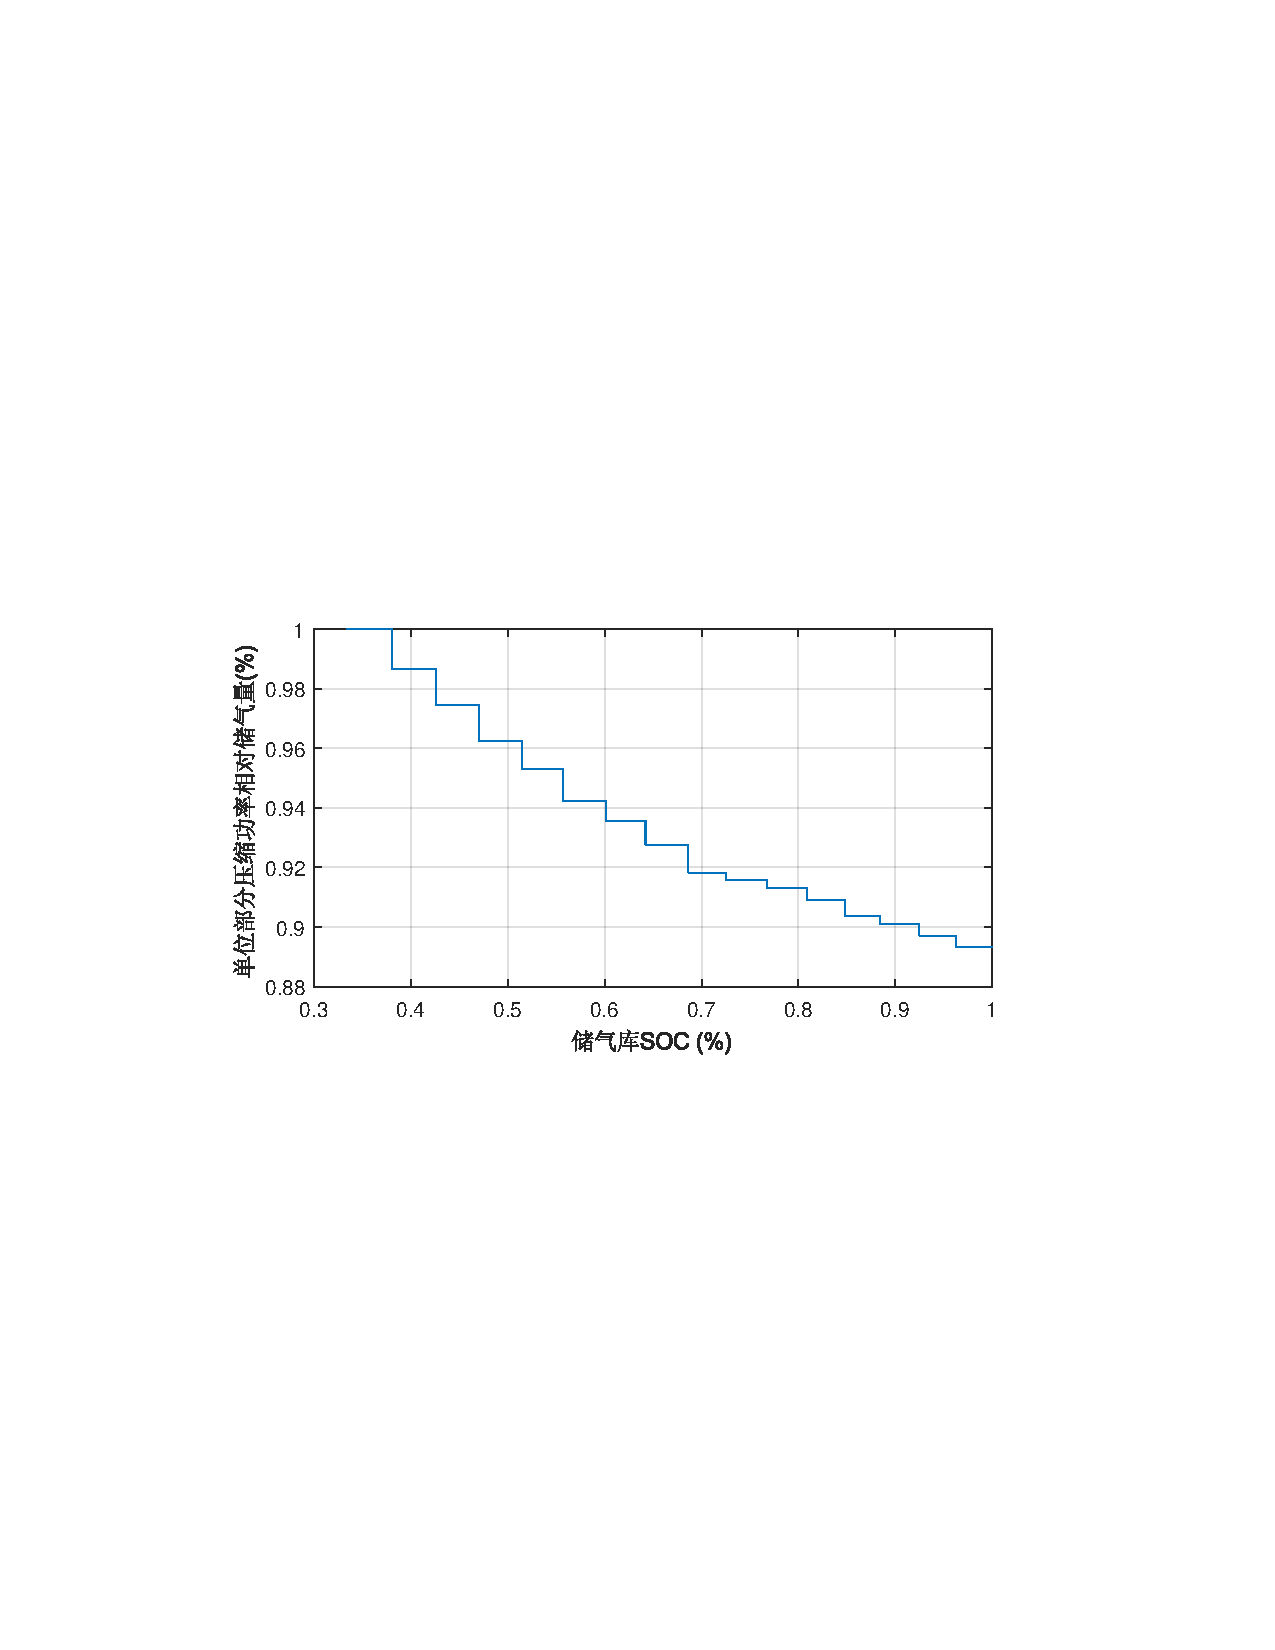
\includegraphics[scale=0.80]{figures/Chap1-8-Compression-SOC-Part-Load.pdf}
  \caption{不同储能水平单位压缩功率(MW)储能量}
  \label{fig:Compression-SOC-Part-Load}
\end{figure}

AA-CAES储能电站在膨胀释能过程中存在与D-CAES电站类似的特性,但相比D-CAES电站而言,AA-CAES电站用压缩储能阶段收集的空气压缩热能代替燃料补燃,其储能水平由储气库储气水平(决定透平入口空气压力)与储热罐储热水平(影响透平入口空气温度)同时决定。由第~\ref{sec:part-load-energy-he}节分析可知,压缩储能阶段收集的压缩热能受换热器的部分负载特性影响明显,从而导致AA-CAES电站释能发电环节的运行灵活性稍低于D-CAES电站。为将组件级的部分负载运行特性嵌入AA-CAES 系统级的宽工况运行模型,需要准确刻画各组件的部分负载运行特性对AA-CAES内部压力势能与压缩热能的存储与消耗水平的集中影响。

\subsection{内部势能-热能双能流耦合关系}
由第\ref{sec:part-load-energy}节中压缩机的部分负载热力学模型(\ref{equ:comp-real-temp-2})-(\ref{equ:comp-mid-var-2})及储气库的热力学动态模型(\ref{equ:Air-tank-model-G})可知,压缩功率对储气库的影响是通过注入空气增加储气量(空气压力势能),膨胀功率对储气库的影响是通过消耗空气减少储气量。另一方面,存储压缩热能的储热系统与压缩侧(或膨胀侧)的耦合来源于压缩侧(或膨胀侧)的换热器。因此,我们可以从换热器与压缩机(或膨胀机)间的热力学耦合关系来建立AA-CAES内部空气压力势能与压缩热能间的解耦存储与耦合释能关系。

本文以压缩储能过程中内部空气势能与压缩热能双能流间的解耦存储关系为例进行分析,膨胀释能过程中内部压力势能与压缩热能间的耦合释能关系与之类似。由式(\ref{equ:turb-power-all})可知,压缩机消耗的功率由空气质量流率及压缩机的入口与出口空气温度决定;由式(\ref{eq:he-comp-temp-out})可知,换热器的换热量由换热器入口与出口温度及质量流率决定。另一方面,储热量由换热器收集或消耗的热功率决定,为此只要合理刻画压缩机耗功与换热器收集的热功率间的关系即可建立内部空气压力势能与空气压缩热能间的解耦存储关系。

为了给出设计工况下压缩机(电)功率与换热器(热)功率间的量化关系,我们暂时假定换热器换热充分,每级压缩机入口空气温度相同(如文献\inlinecite{TICC-15,TICC-16}中的试验系统),考虑到压缩机出口温度等于相邻换热器入口温度(参见图~\ref{fig:CAES-thermal-struc} 所示~AA-CAES~结构及边界条件),从而换热器的换热功率大致等于压缩机消耗的电功率(亦可参见\ref{sec:chap2-bound-measure}节中的仿真分析)\footnote{出现压缩机耗功与换热器收集热功率相等现象的一个原因是,一般假定空气的定压比热容为定值,实际中二者并不相同。}。实际运行过程中,由于受组件部分负载特性及系统宽工况运行要求的影响,压缩机的电功率与储热系统的储热功率(换热器的集热功率)间的关系是时变的,同时还受AA-CAES系统本身结构参数以及运行方式的影响。因此,AA-CAES内部压力势能与压缩热能间的解耦存储与耦合释能关系可分别通过压缩侧与膨胀侧换热器的特性表示为,
\begin{subequations}
\label{equ:coup-heat-power}
\begin{gather}
\varphi ({P_t^c,h_t^c}) = 0 \label{equ:coup-heat-power-char}\\
\phi ({P_t^d,h_t^d}) = 0 \label{equ:coup-heat-power-disc}
\end{gather}
\end{subequations}
其中,$P_t^c$与$P_t^d$分别为时段$t$(所有)压缩机消耗与(所有)膨胀机输出的电功率,实际上其值分别与第\ref{cha:simulation}章中对应时刻的压缩机耗功$W_{c}$ 与膨胀机输出功$W_{e}$ 相同\footnote{第2章针对压缩机、膨胀机及换热器等建立稳态热力学仿真模型时并未明确引入时间下标$t$,从本章开始我们将研究含第2章中各通用组件的AA-CAES不同实现或应用形式在电力系统中的运行建模、调度运行及市场运营等问题,相应模型一般会直接在第2章相关变量的基础上加入时间下标$t$,而不做过多解释。 同时,我们假定一个运行时段内各个时刻各物理量不发生变化,而时段的大小视所分析问题的不同而有所差别。此外,在不引起混淆的情况下,我们允许对时刻与时段的混用。};$h_t^c$ 与$h_t^d$ 分别为储能阶段注入储热系统的热功率与释能阶段消耗的热功率,实际上其值可由第\ref{cha:simulation}章中的HTF比热容$c_p^{HTF}$,质量流率($\dot m_e^{HTF}$,$\dot m_c^{HTF}$),以及对应的HTF温度($T^{TES}, T_{c,HX}^{HTF, Merge}, T_{e,HX}^{Merge},T_{cool}^{HTF}$)等计算而得。(\ref{equ:coup-heat-power-char})表示储能过程中储热功率与储电功率(即压缩机电功率)间的耦合关系,间接刻画了压力势能与压缩热能的解耦存储关系;(\ref{equ:coup-heat-power-disc}) 表示释能过程中耗热功率与放电功率(即膨胀机电功率)间的耦合关系,间接刻画了压力势能与压缩热能的耦合释能关系。

特别地,势能与热能双能流间耦合关系(\ref{equ:coup-heat-power})的特殊形式可表示为,
\begin{subequations}
\label{equ:coup-heat-power-spe}
\begin{gather}
h_t^c = \varphi ({P_t^c})P_t^c \label{equ:coup-heat-power-char-spe}\\
P_t^d = \phi ({P_t^d})h_t^d  \label{equ:coup-heat-power-disc-spe}
\end{gather}
\end{subequations}
其中,$\varphi ({P_t^c})$与$\phi ({P_t^d})$分别为储能过程与释能过程中所有换热器部分负载运行时的集中(等效)效能,也分别表征了AA-CAES 压缩储能过程中将电功率转化为热功率以及膨胀释能过程中将热功率转化为电功率的能力,与热泵等电热转换设备的效率具有类似的物理意义。

本章后续使用$P_t^c$与$P_t^d$表征AA-CAES与电力系统的(电)功率输入与(电)功率输出接口,实现对$W_c$与$W_e$及压缩机与膨胀机内部热力学特性的封装;同时,也采用$h_t^c$ 与$h_t^d$ 实现对内部HTF热力学状态相关信息的封装。通过引入隐函数$\varphi ({P_t^c,h_t^c})$与$\phi ({P_t^d,h_t^d})$,我们将第2章中复杂的压力势能与压缩热能间的热力学耦合关系集中体现于$\varphi(\cdot) $与$\phi(\cdot)$上,后续应用只需关注接口信息($ P_t^c$、$P_t^d$、$h_t^c$、 $h_t^d$)以及$\varphi(\cdot)$与$\phi(\cdot)$ 的具体形式即可。换言之,给定任一外部应用的可行功率接口信息,AA-CAES便能通过(外部无需了解的)内部的热力学状态参数实现该功率接口。

\subsection{外部电功率与储/耗气量的耦合关系}
AA-CAES组件的部分负载特性对储气库储气水平的整体影响表现在式(\ref{equ:air-SOC-energy})中压缩功率(或膨胀功率)受背压(或入口压力)影响导致的单位压缩(或膨胀)电功率储气量(或耗气量)的部分负载特性。为此,本文用$m_t^{ch}$ 与$m_t^{dis}$ 分别表示计及压缩机与膨胀机的部分负载特性时,时段$t$ 进入与流出储气库的高压空气质量,且满足,
\begin{subequations}
\label{equ:coup-mass-SOC}
\begin{gather}
m_t^{ch} = \Gamma({P_t^c,A_t^{soc}})P_t^c\label{equ:coup-mass-SOC-char}\\
m_t^{dis} = \Psi({P_t^d,A_t^{soc}})P_t^d \label{equ:coup-mass-SOC-disc}
\end{gather}
\end{subequations}
其中,$A_t^{soc}$ 为储气库无量纲储气水平;函数$\Gamma(\cdot)$ 建立了储能过程中压缩功率$P_t^c$ 与进气量$m_t^{ch}$间的关系;函数$\Psi(\cdot)$ 建立了释能过程中膨胀功率$P_t^d$与耗气量$m_t^{dis}$间的关系,即函数$\Gamma (\cdot)$与$\Psi(\cdot)$分别等效表征了单位压缩功率的进气量与单位膨胀功率的耗气量,反映了压缩机与膨胀机的部分负载运行特性与储气库动态特性间的耦合关系。

一般地,函数$\Gamma(\cdot)$与函数$\Psi(\cdot)$的具体表达式依赖于第\ref{cha:simulation}章中引入的AA-CAES的四种运行模式,即常压-常压、常压-滑压、滑压-常压、滑压- 滑压等。以函数$\Gamma(\cdot)$为例,当不存在储气库入口侧节流阀(见\ref{fig:CAES-thermal-struc}),即压缩侧采用滑压运行策略时,压缩储能过程中压缩机的背压为储气库实时压力,函数$\Gamma(\cdot)$ 与$A_t^{soc}$有关;当存在入口侧节流阀,即压缩机采用常压运行策略时,压缩机的部分负载运行特性不受储气库压力影响,函数$\Gamma(\cdot)$ 退化为$\Gamma (P_t^c)$ ,与$A_t^{soc}$ 无关。特别地,当AA-CAES处于额定工况运行,且储气库入口与出口均存在节流阀(常压-常压运行)时,$\Gamma(\cdot)$与$\Psi(\cdot)$变为固定系数,式(\ref{equ:coup-mass-SOC})将退化为常效率模型。由此可见,外部输入/输出电功率与储气库进/出气量间的通用耦合关系(\ref{equ:coup-mass-SOC})涵盖了AA-CAES系统的典型运行模式。

\subsection{热力学特性曲线簇}
基于前述分析,储能电站运行时的AA-CAES系统级的宽工况特性,可由基于换热器视角表示的内部势能-热能双能流耦合关系函数$\varphi$与$\phi$,以及基于压缩机与膨胀机视角表示的外部输入/输出电功率与储气/耗气量间耦合关系的函数$\Gamma $与$\Psi$集中表示。本文将($\Gamma$, $\Psi$, $\varphi$, $\phi$)称为表征AA-CAES宽工况运行特性的热力学特性曲线簇,即AA-CAES对外部应用提供的接口函数,其可基于第\ref{cha:simulation}章中计及组件部分负载特性的AA-CAES宽工况热力学仿真模型产生,或由实际AA-CAES储能电站的运行数据拟合给定。其理性在于,电力系统调度等应用处理火电机组的复杂运行特性时,一般会采用常系数(未考虑火电机组宽工况特性)或采用基于输入输出特性曲线的变系数,而该特性曲线通常由火电厂实测运行数据拟合给定。在实际运行过程中,热力学特性曲线簇($\Gamma$, $\Psi$, $\varphi$, $\phi$)中的函数$\Gamma(\cdot)$与$\Psi(\cdot)$受AA-CAES储能电站运行模式的影响,而函数$\varphi(\cdot)$与$\phi(\cdot)$则受供能模式影响。
%以下基于第2章的仿真系统给出该特性曲线簇的典型形状。

%\subsection{仿真参数设置}
%本节采用图~\ref{fig:CAES-thermal-struc}所示的两级压缩两级膨胀~AA-CAES~储能电站,以典型滑压-常压运行模式分析宽工况热力学特性曲线,为面向智能电网应用的~AA-CAES~构建不失建模准确性的能量及备用模型提供基础。本节以江苏金坛~60~MW AA-CAES储能电站设计参数\footnote{部分参数细节与实际参数有所出入,但不影响本章建模的思路。}为例,进行分析。

%\begin{table}[htb]
%  \centering
%  \begin{minipage}[t]{0.70\linewidth} % 如果想在表格中使用脚注,minipage是个不错的办法
%  \caption{60MW AA-CAES 储能电站空气压缩机额定参数}
%  \label{tab:CAES-60-para-comp}
%    \begin{tabularx}{\linewidth}{ccccccc}
%      \toprule[1.5pt]
%      \multirow{2}*{\heiti 压缩级} &  \multirow{2}*{\heiti 增压比} &  \multirow{2}*{\heiti 绝热效率(\%)} &  \multicolumn{2}{c}{\heiti 压力(Mpa)} & \multicolumn{2}{c}{\heiti 温度($^{\circ}$C)}\\
%      \cline{4-7}
%        &   &   &  进气 & 排气 & 进气 & 排气 \\
%     \midrule[1pt]
%      一级 & 3.545 & 72.8 & 0.099 & 0.351  & 25 & 143 \\
%      二级 & 2.668 & 78.6 & 0.351 & 0.913  & 45 & 145 \\
%      三级 & 2.677 & 82.2 & 0.913 & 2.392  & 45 & 149 \\
%      \bottomrule[1.5pt]
%    \end{tabularx}
%  \end{minipage}
%\end{table}

%\begin{table}[htb]
%  \centering
%  \begin{minipage}[t]{0.75\linewidth} % 如果想在表格中使用脚注,minipage是个不错的办法
%  \caption{60MW AA-CAES储能电站空气透平膨胀机额定参数}
%  \label{tab:CAES-60-para-turb}
%    \begin{tabularx}{\linewidth}{ccccccc}
%      \toprule[1.5pt]
%      \multirow{2}*{\heiti 膨胀级} &  \multirow{2}*{\heiti 膨胀比} &  \multirow{2}*{\heiti 绝热效率(\%)} &  \multicolumn{2}{c}{\heiti 压力(Mpa)} & \multicolumn{2}{c}{\heiti 温度($^{\circ}$C)}\\
%      \cline{4-7}
%        &   &   &  进气 & 排气 & 进气 & 排气 \\
%     \midrule[1pt]
%      一级 & 3.545 & 87.9 & 3.00 & 1.02  & 100 & 12 \\
%      二级 & 2.668 & 87.0 & 1.01 & 0.34  & 100 & 13 \\
%      \bottomrule[1.5pt]
%    \end{tabularx}
%  \end{minipage}
%\end{table}
%
%\begin{table}[htb]
%  \centering
%  \begin{minipage}[t]{0.85\linewidth} % 如果想在表格中使用脚注,minipage是个不错的办法
%  \caption{60MW AA-CAES 储能电站压缩侧换热器额定参数}
%  \label{tab:CAES-60-para-he-comp}
%    \begin{tabularx}{\linewidth}{cccccccc}
%      \toprule[1.5pt]
%      \multirow{2}*{\heiti 换热级} &  \multicolumn{2}{c}{\heiti 空气温度($^{\circ}$C)} &  \multicolumn{2}{c}{\heiti 冷却水温度($^{\circ}$C)}  & \multicolumn{2}{c}{\heiti 温差($^{\circ}$C)} & \multirow{2}*{\heiti 水侧流量(kg/h)}\\
%      \cline{2-7}
%        &  入口 & 出口  & 入口 & 出口  & 热端  & 冷端 &   \\
%     \midrule[1pt]
%      一级 & 143 & 45 & 35 & 120  & 23 & 10  & 451.091\\
%      二级 & 145 & 45 & 35 & 120  & 25 & 10 & 462.841\\
%      三级 & 149 & 45 & 35 & 120  & 29 & 10 & 487.968 \\
%      \bottomrule[1.5pt]
%    \end{tabularx}
%  \end{minipage}
%\end{table}
%
%\begin{table}[htb]
%  \centering
%  \begin{minipage}[t]{0.85\linewidth} % 如果想在表格中使用脚注,minipage是个不错的办法
%  \caption{60MW AA-CAES 储能电站膨胀侧换热器额定参数}
%  \label{tab:CAES-60-para-he-turb}
%    \begin{tabularx}{\linewidth}{cccccccc}
%      \toprule[1.5pt]
%      \multirow{2}*{\heiti 换热级} &  \multicolumn{2}{c}{\heiti 空气温度($^{\circ}$C)} &  \multicolumn{2}{c}{\heiti 加热水温度($^{\circ}$C)}  & \multicolumn{2}{c}{\heiti 温差($^{\circ}$C)} & \multirow{2}*{\heiti 水侧流量(kg/h)}\\
%      \cline{2-7}
%        &  入口 & 出口  & 入口 & 出口  & 热端  & 冷端 &   \\
%     \midrule[1pt]
%      一级 & -10 & 100 & 120 & 35  & 20 & 45  & 2841\\
%      二级 & 12  & 100 & 120 & 35  & 20 & 23  & 2212\\
%      三级 & 13  & 100 & 120 & 35  & 20 & 23  & 2169\\
%      \bottomrule[1.5pt]
%    \end{tabularx}
%  \end{minipage}
%\end{table}

\section{宽工况双SOC建模框架及典型模型}
\label{sec:dual-SOC}
前已提及,第~\ref{cha:simulation}章建立的宽工况热力学仿真模型主要用于热力学特性分析,若直接用于电力系统中AA-CAES储能电站的运行分析,将导致模型异常复杂,不便于实际工程所采纳。本节在第\ref{sec:chap3-aa-caes-sim}节提出的宽工况热力学特性曲线簇的基础上,借鉴电池储能的荷电水平(State-of-charge,SOC)建模思想,将
从能量转换类模块(压缩机与空气透平)及能量转移类模块(换热器)视角得出的热力学特性曲线簇“嵌入”内部能量存储类模块(储气库与储热罐)的SOC方程中,建立面向电力系统应用的AA-CAES宽工况双SOC建模体系及具体模型,其基本框架如图~\ref{fig:AA-CAES-Part-Load-Model}所示。

\begin{figure}[H] % use float package if you want it here
  \centering
  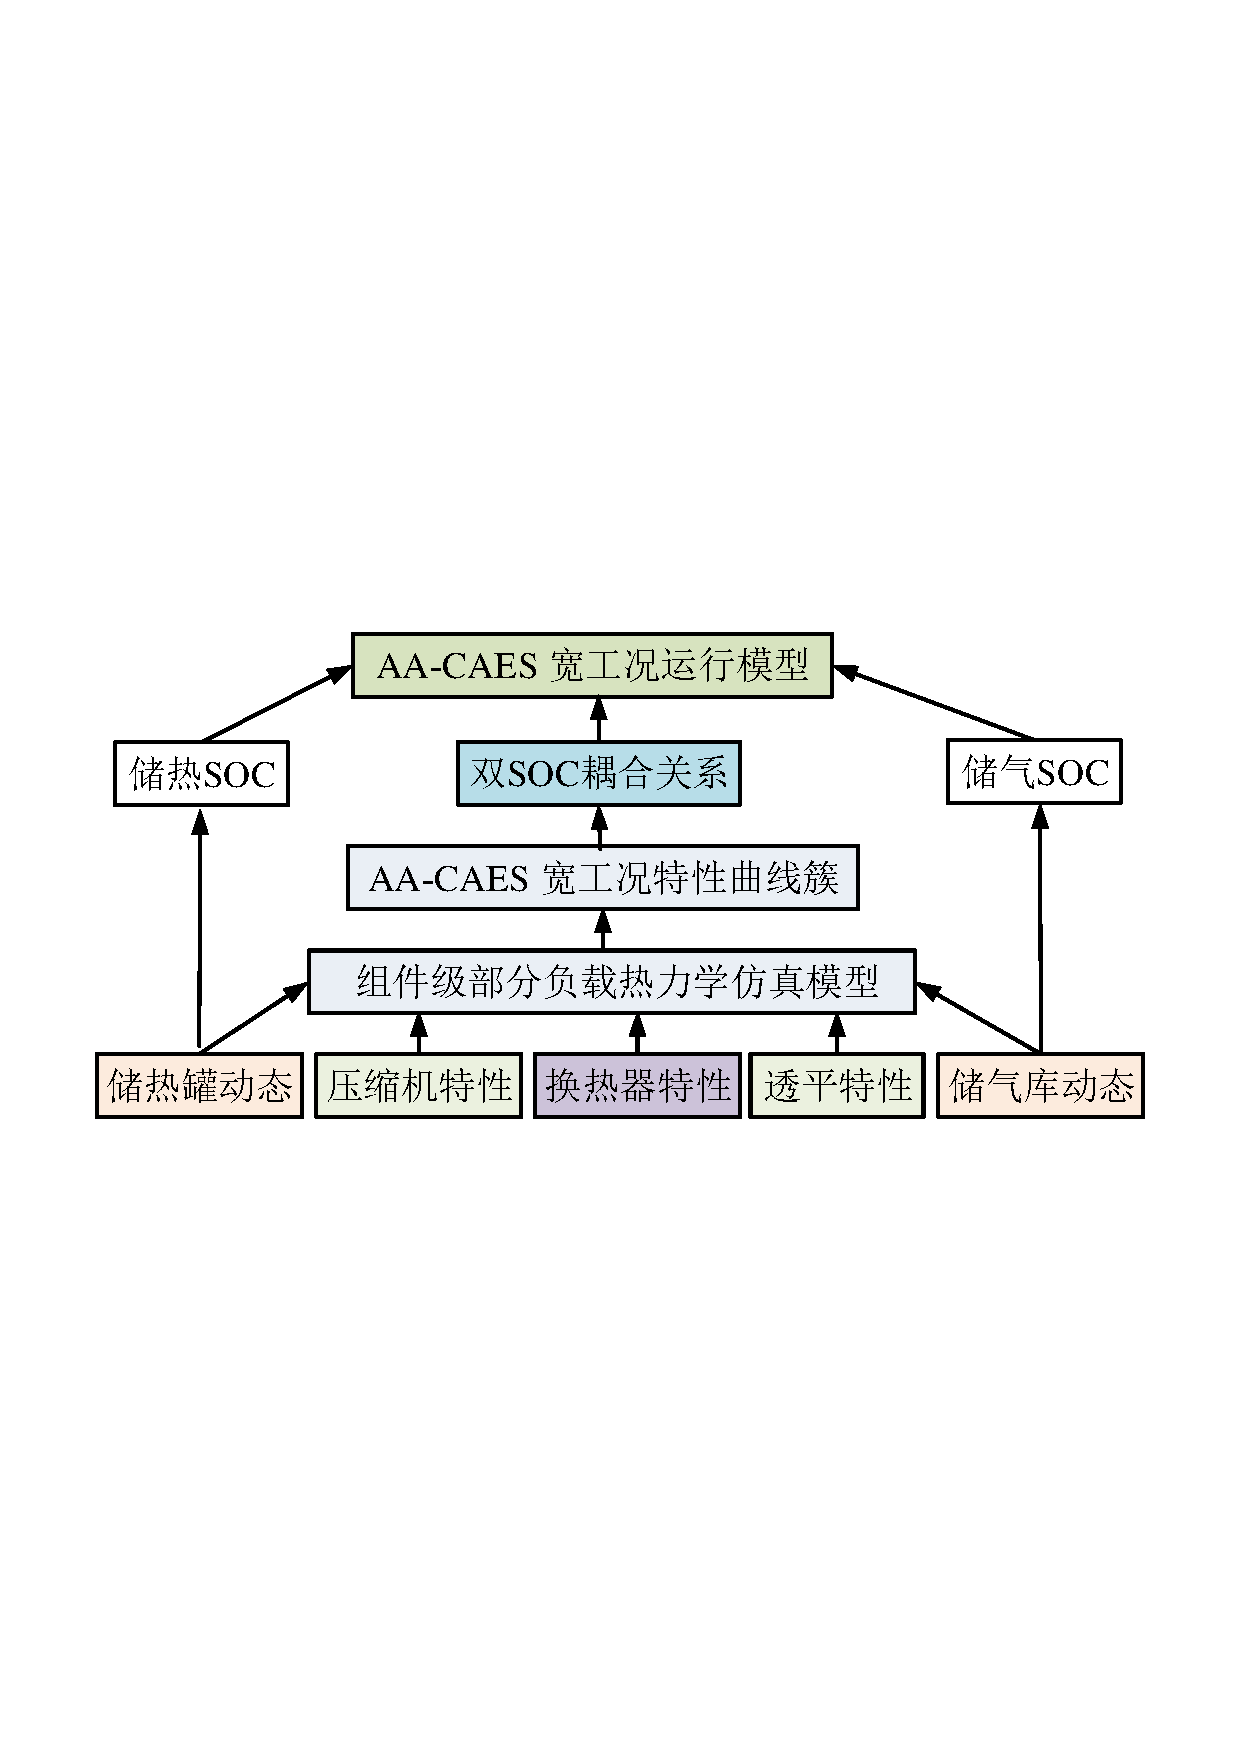
\includegraphics[scale=0.60]{figures/Chap3-2-AA-CAES-Part-Load-Model.pdf}
  \caption{AA-CAES储能电站的双SOC模型建模框架}
  \label{fig:AA-CAES-Part-Load-Model}
\end{figure}

运用双SOC模型建模框架,我们可以得出面向电力规划、调度运行及市场运营等应用的AA-CAES储能电站的系列模型。本节将重点给出双SOC能量模型、双SOC能量与备用模型,以及能量与备用模型的扩展形式,以说明宽工况双SOC建模框架的应用方法。

\subsection{双SOC能量模型}
\label{sec:dual-SOC-energy}
一般地,储气库的储气SOC可以采用储气压力构建,如文献\inlinecite{CAES-IES-16-Rui}中采用的储气库模型。 然而,基于压力动态描述的储气SOC模型难以将第
\ref{cha:simulation}章中给出的面向AA-CAES热力学特性仿真的通用储气库、等温储气库及绝热储气库等模型纳入统一框架。换言之,采用不同的储气库仿真模型时,影响储气库压力动态的因素不同,采用G模型时储气库压力受进/出气量以及储气库内空气与周围环境传热过程的影响;采用VT与VA模型时,压力动态仅受进/出空气的热力学状态影响。

本节基于储气库中的空气质量动态建立储气SOC模型,其出发点在于,不论储气库采用G模型、VT或VA模型,质量动态方程仅受进/出气量影响,且具有简洁统一的形式(参见
(\ref{equ:Air-tank-model-G})、(\ref{equ:Air-tank-model-VT})、(\ref{equ:Air-tank-model-VA})),%(可参见(\ref{equ:Air-tank-model-G-M})、(\ref{equ:Air-tank-model-VT-M}) 及(\ref{equ:Air-tank-model-VA-M})),
同时也便于与第\ref{sec:chap3-aa-caes-sim}节中的宽工况特性曲线簇实现有机结合。事实上,针对传统D-CAES电站,基于储气库空气质量构建储气SOC的思路已被逐渐接受,如文献\inlinecite{CAES-Bilinear-17,CAES-Reserve-Bid-Therm-16}。

基于储气库热力学动态模型(\ref{equ:Air-tank-model-G})-(\ref{equ:Air-tank-model-VA}),可将储气SOC表示为,
\begin{subequations}
\label{equ:air-SOC-energy}
\begin{gather}
A_{t + 1}^{soc} = A_t^{soc}(1-\gamma_{A}) + \frac{1}{{{A_{\max}^{circ}}}}({m_t^{ch} - m_t^{dis}})\label{equ:air-SOC-energy-balance}\\
A_{\min }^{soc} \le A_t^{soc} - \frac{{m_t^{dis}}}{{{{\rm{A}}_{\max }^{circ}}}}\\
{\rm{A}}_t^{soc} + \frac{{m_t^{ch}}}{{{{\rm{A}}_{\max }^{circ}}}} \le A_{\max }^{soc}
\end{gather}
\end{subequations}
其中,$\gamma_{A}$为表征储气库漏气特性的常数,一般可设为0-0.02,基于第2章不计及储气库漏气问题的假设,此处取为0;${A_{\max}^{circ}}$ 为储气库最大循环空气质量,由储气库压力上下限($p_{as}^{min}$, $p_{as}^{max}$) 及体积$V_{as}$等决定;${{A}}_t^{soc}$ 为时刻$t$的储气百分数;${{A}}_{\min }^{soc}$ 与 ${{A}}_{\max }^{soc}$ 分别为维持最小与最大储气压力所需的空气质量百分数。
 %$m_t^{ch}$ 与$m_t^{dis}$分别表示进入与流出储气库的空气质量,受宽工况运行影响。由第~\ref{sec:chap3-aa-caes-sim}节分析可知,宽工况运行模式下,AA-CAES储能电站单位压缩功率对应的 $m_t^{ch}$ 将减小,单位膨胀功率所需的$m_t^{dis}$ 将增大。

类似地,基于储热系统的热力学动态模型(\ref{equ:TES-HTF-temp}),可将储热SOC表示为\footnote{若需考虑AA-CAES对外的供热功率(假定用收集的压缩热供热),只需在(\ref{equ:TES-SOC-energy-balance})中新增一项$h_t^{g}$即可。},
\begin{subequations}
\label{equ:TES-SOC-energy}
\begin{gather}
H_{t + 1}^{soc} = H_t^{soc}(1-\gamma_{H}) + \frac{1}{{{H_{\max}^{circ}}}}({h_t^c\Delta t - h_t^d\Delta t})\label{equ:TES-SOC-energy-balance}\\
H_{\min }^{soc} \le H_t^{soc} - \frac{{h_t^d\Delta t}}{{{H_{\max }^{circ}}}}\\
H_t^{soc} + \frac{{h_t^c\Delta t}}{{{H_{\max }^{circ}}}} \le H_{\min }^{soc}
\end{gather}
\end{subequations}
其中, $\gamma_{H}$表征储热罐与周围环境的换热过程引起的储热量损耗,其大小与储热罐特性有关,可假定为常数,当储热罐采用绝热模型时,其值为0;${H_{\max}^{circ}}$ 为储热系统最大储热量,一般需根据应用场景进行设置,如热电联供模式下的最大储热量比仅供电模式要大;$H_t^{soc}$为储热相对百分数;${{H}}_{\min }^{soc}$与${{H}}_{\max }^{soc}$ 分别为最小与最大储热百分数;$\Delta t$ 为时间间隔,其它参数物理意义与式(\ref{equ:air-SOC-energy})类似。

在AA-CAES储能电站的压缩储能过程中,通过压力势能与压缩热能的解耦存储,压缩功率同时改变储气SOC与储热SOC的状态;膨胀释能过程中,通过压力势能与压缩热能的耦合释能,储气SOC与储热SOC共同影响膨胀功率。因此,通过引入含有压缩功率与膨胀功率接口的宽工况热力学特性曲线簇($\Gamma$, $\Psi$, $\varphi$, $\phi$),即可实现储气SOC与储热SOC的耦合。

综上,AA-CAES储能电站的宽工况双SOC能量模型由(\ref{equ:coup-heat-power})、(\ref{equ:coup-mass-SOC})、(\ref{equ:air-SOC-energy})及(\ref{equ:TES-SOC-energy})构成,其对电力系统调度等外部应用提供了功率接口($P_t^c$, $P_t^d$)以及储能水平($A_t^{soc}$, $H_t^{soc}$)。

\subsection{双~SOC~能量与备用模型}
\label{sec:dual-SOC-Reserve}

在第\ref{sec:dual-SOC-energy}节中我们建立了AA-CAES储能电站的宽工况双SOC能量模型。事实上,AA-CAES储能电站可为电网提供容量备用等灵活性支撑。为此,可将双SOC 能量模型扩展为计及备用特性的双~SOC~能量与备用模型。我们仅考虑正负荷备用\footnote{该设定的合理性主要体现在系统中备用主要是用于缓解调峰或机组/线路临时故障退出引起的负荷难以满足等问题。},即通过减少压缩机消耗的电功率$P_t^c$与增加透平输出的电功率$P_t^d$来提供灵活性支撑。由图\ref{fig:CAES-AS-Overview} 分析可知,压缩储能过程能提供旋转备用$P_t^{c,sr}$,膨胀释能过程可同时提供旋转备用$P_t^{d,sr}$ 与非旋转备用$P_t^{d,nr}$。为了刻画AA-CAES的备用容量接口,我们定义如下的等效压缩功率与等效膨胀功率,
\begin{subequations}
\label{equ:def-Pc-Pd-eq}
\begin{gather}
P_t^{c,eq} = P_t^c - P_t^{c,sr}\label{equ:def-Pc-eq}\\
P_t^{d,eq} = P_t^d + P_t^{d,sr} + P_t^{d,nr}\label{equ:def-Pd-eq}
\end{gather}
\end{subequations}
其中,$P_t^{c,eq}$表示计及压缩机的旋转备用容量的等效压缩功率;$P_t^{d,eq}$表示计及空气透平旋转备用及非旋转备用容量的等效膨胀功率。

计及备用特性后,储气SOC模型可调整为,
\begin{subequations}
\label{equ:air-SOC-reserve}
\begin{gather}
A_{t + 1}^{soc} = A_t^{soc}(1-\gamma_A) + \frac{1}{{{A_{\max }^{circ}}}}({m_t^{ch} - m_t^{dis}})\\
A_{\min }^{soc} \le A_t^{soc} - \frac{{m_t^{dis,eq}}}{{{A_{\max}^{circ}}}}\label{equ:air-SOC-reserve-diff}\\
{{A}}_t^{soc} + \frac{{m_t^{ch}}}{{{{\rm{A}}_{\max}^{circ}}}} \le A_{\max }^{soc}
\end{gather}
\end{subequations}
相应地,储热SOC模型可调整为\footnote{若需考虑AA-CAES热电联供时具有的热功率备用能力,只需稍微修改(\ref{equ:TES-SOC-reserve})即可。},
\begin{subequations}
\label{equ:TES-SOC-reserve}
\begin{gather}
H_{t + 1}^{soc} = H_t^{soc}(1-\gamma_H) + \frac{1}{{{H_{\max}^{circ}}}}({h_t^c\Delta t - h_t^d\Delta t})\label{equ:TES-SOC-reserve-S1}\\
H_{\min }^{soc} \le H_t^{soc} - \frac{{h_t^{d,eq}\Delta t}}{{{H_{\max}^{circ}}}}\label{equ:TES-SOC-reserve-diff}\\
H_t^{soc} + \frac{{h_t^c\Delta t}}{{{H_{\max}^{circ}}}} \le H_{\max }^{soc}
\end{gather}
\end{subequations}
其中,$m_t^{dis,eq}$与$h_t^{d,eq}$分别为对应于等效膨胀功率$P_t^{d,eq}$的耗气量与耗热功率,二者分别满足,
\begin{subequations}
\label{equ:coup-mass-heat-SOC-reserve}
\begin{gather}
m_t^{dis,eq} = \Psi ({P_t^{d,eq},A_t^{soc}})P_t^{d,eq}\label{equ:coup-mass-SOC-reserve-S3}\\
\phi ({P_t^{d,eq},h_t^{d,eq}}) = 0\label{equ:coup-heat-power-reserve-S3}
\end{gather}
\end{subequations}

需要强调的是,在双SOC能量与备用模型中的储气及储热SOC与双SOC能量模型的储气及储热SOC的不同之处仅在于(\ref{equ:air-SOC-reserve-diff})与(\ref{equ:TES-SOC-reserve-diff}),其原因在于不计及备用容量的实际调用时,备用容量只受到储气与储热SOC的上下界影响,而不影响储气SOC与储热SOC方程。在膨胀释能过程中,提供备用容量时需要增大膨胀功率,其备用容量受到储气量下限及储热量下限的影响;在压缩储能过程中,提供备用容量时由于需要减小压缩功率,备用容量不受储气量上限与储热量上限的影响。

综上,AA-CAES储能电站的宽工况双SOC能量与备用模型由(\ref{equ:coup-heat-power})、(\ref{equ:coup-mass-SOC})、(\ref{equ:def-Pc-Pd-eq})、(\ref{equ:air-SOC-reserve})、(\ref{equ:TES-SOC-reserve})及(\ref{equ:coup-mass-heat-SOC-reserve})组成,其对外部电力系统应用提供了功率接口($P_t^c$,$P_t^d$),容量备用接口($P_t^{c,sr}$,$P_t^{d,sr}$,$P_t^{d,nr}$),以及储能水平($A_t^{soc}$, $H_t^{soc}$)。

\subsection{能量与备用模型的扩展}
\label{sec:dual-SOC-Reserve-exten}
第\ref{sec:dual-SOC-Reserve}节中所建的双~SOC~能量与备用模型中未考虑实际运行(或实时市场)中备用调度对AA-CAES 储能电站双SOC状态的影响,一般用于含储能的电力系统灵活性评估或容量规划、不计及备用调用的储能电站市场运营等问题。本节旨在进一步扩展双~SOC~能量与备用模型,以计及备用容量的调用对储气与储热SOC状态的影响。

为刻画计及备用容量的实际调用时,AA-CAES的双SOC模型接口,我们定义如下的计及备用调用的等效压缩功率与等效膨胀功率,
\begin{subequations}
\label{equ:def-power-relation}
\begin{gather}
P_t^{c,Ev} = P_t^c - P_t^{c,sr}u_t^{sr}\\
P_t^{d,Ev} = P_t^d + P_t^{d,sr}u_t^{sr} + P_t^{d,nr}u_t^{nr}
\end{gather}
\end{subequations}
其中,$u_t^{sr}$与$u_t^{nr}$分别为表征旋转备用与非旋转备用容量调用状态的布尔量;$P_t^{c,Ev}$为计及备用容量调用($P_t^{c,sr}$)的等效压缩功率;$P_t^{d,Ev}$为计及备用容量($P_t^{d,sr}$,$P_t^{d,nr}$)调用的等效膨胀功率。


计及备用调用后,储气SOC模型可修正为,
\begin{subequations}
\label{equ:air-SOC-reserve-exten}
\begin{gather}
A_{t + 1}^{soc} = A_t^{soc}(1-\gamma_A) + \frac{1}{{{A_{\max}^{circ}}}}({m_t^{ch,Ev} - m_t^{dis,Ev}})\\
A_{\min }^{soc} \le A_t^{soc} - \frac{{m_t^{dis,Ev}}}{{{A_{\max}^{circ}}}}\\
{\rm{A}}_t^{soc} + \frac{{m_t^{ch}}}{{{{\rm{A}}_{\max}^{circ}}}} \le A_{\max }^{soc}
\end{gather}
\end{subequations}
相应地,储热SOC模型可修正为,
\begin{subequations}
\label{equ:TES-SOC-reserve-exten}
\begin{gather}
H_{t + 1}^{soc} = H_t^{soc}(1-\gamma_H) + \frac{1}{{{H_{\max}^{circ}}}}({h_t^{c,Ev}\Delta t - h_t^{d,Ev}\Delta t})\\
H_{\min }^{soc} \le H_t^{soc} - \frac{{h_t^{d,Ev}\Delta t}}{{{H_{\max}^{circ}}}}\\
H_t^{soc} + \frac{{h_t^c\Delta t}}{{{H_{\max}^{circ}}}} \le H_{\max }^{soc}
\end{gather}
\end{subequations}
其中,$m_t^{ch,Ev}$与$m_t^{dis,Ev}$分别为等效压缩功率$P_t^{c,Ev}$与等效膨胀功率$P_t^{d,Ev}$对应的进气量与耗气量;$h_t^{c,Ev}$与$h_t^{d,Ev}$分别为$P_t^{c,Ev}$与$P_t^{d,Ev}$对应的储热功率及耗热功率。特别地,计及备用容量的调用后,内部热力学特性间的耦合关系(宽工况特性曲线方程)需调整为,
\begin{subequations}
\label{equ:coup-heat-power-reserve-exten}
\begin{gather}
m_t^{ch,Ev} = \Gamma ({P_t^{c,Ev},A_t^{soc}})P_t^{c,Ev}\\
m_t^{dis,Ev} = \Psi ({P_t^{d,Ev},A_t^{soc}})P_t^{d,Ev}\\
\varphi ({P_t^{c,Ev},h_t^{c,Ev}}) = 0\\
\phi ({P_t^{d,Ev},h_t^{d,Ev}}) = 0
\end{gather}
\end{subequations}

综上,计及备用调用后,AA-CAES储能电站双SOC能量与备用扩展模型由(\ref{equ:def-power-relation})、(\ref{equ:air-SOC-reserve-exten})、(\ref{equ:TES-SOC-reserve-exten})及(\ref{equ:coup-heat-power-reserve-exten})组成,其对外部电力系统应用提供了功率接口($P_t^c$,$P_t^d$)、容量备用接口($P_t^{c,sr}$,$P_t^{d,sr}$,$P_t^{d,nr}$)、储能水平($A_t^{soc}$, $H_t^{soc}$),以及备用容量在实际运行中的调用状态($u_t^{sr}$, $u_t^{nr}$)。

\section{计及AA-CAES宽工况特性的风-储协同调度运行}
\label{sec:chap3-wind-ESS-operation}
本节基于第\ref{sec:dual-SOC}节中储能电站的宽工况双SOC能量模型,分析AA-CAES的宽工况运行特性对风电与储能电站协同系统(如图\ref{fig:AA-CAES-Stru-Felixibity} 中配置方案)运行特性的影响。

\subsection{协同发电能力分析模型}
本节假定风- 储协同系统以最大化风电上网电量或风电容量因子(Capacity Factor, CF)为目标。除满足第\ref{sec:dual-SOC}节中的双SOC能量模型之外,风-储协同运行需满足如下的运行限制,
\begin{subequations}
\label{eq:WT-CAES-Power-Limit}
\begin{gather}
u_t^c + u_t^d \le 1,u_t^c,u_t^d \in \left\{ {0,1} \right\}, \forall t\\
P_{\min }^cu_t^c \le P_t^c \le P_{\max }^cu_t^c, \forall t \\
 P_{\min }^du_t^d \le P_t^d \le P_{\max }^du_t^d, \forall t
\end{gather}
\end{subequations}
其中,$u_t^c$ 与 $u_t^d$ 分别为表示压缩储能与膨胀释能运行状态的布尔量;$P_{\max }^c$ 与 $P_{\max }^d$ 分别为压缩机与空气透平的额定功率;$P_{\min }^c$ 与 $P_{\min }^d$ 分别为压缩机与空气透平的最小技术出力。对于AA-CAES储能电站这类宽工况运行特性较为明显的系统,最小技术出力的确定需通过经济性评估等界定,如火电机组按照机组容量的不同,大型机组的最小技术出力一般设定为额定功率的50\%。

为了聚焦于宽工况运行对风-储系统影响的分析,我们假定AA-CAES储能电站仅通过与之协同运行的风电进行储能(参见图\ref{fig:AA-CAES-Stru-Felixibity})。因此,风-储系统系统需满足如下约束,
\begin{equation}
\label{eq:WT-Power-Limit}
P_t^c \le {W_t},P_t^d + {W_t} \le {W_{rated}},\forall t
\end{equation}
其中,$W_t$ 与 $W_{rated}$分别为风电实际出力与额定功率,且满足风机的功率曲线,
\begin{equation}
\label{eq:WT-Power-Curve}
{W_t} = \;\left\{ \begin{array}{l}
{\rm{0}}\;\;\;\;\;\;\;\;\;\;\;\;\;\;\;\;\;{v_t} < {v_{in}}\;\;{v_t} > {v_{out}}\\
{W_{rated}}\frac{{{v_t} - {v_{in}}}}{{{v_{rated}} - {v_{in}}}},\;\;{v_{in}} \le {v_t} \le {v_{rated}}\\
{W_{rated}},\;\;\;\;\;\;\;\;\;\;\;\;\;{v_{rated}} \le {v_t} < {v_{out}}
\end{array} \right.
\end{equation}
其中,$v_t$ 为实际风速;$v_{in}$ ,$v_{rated}$,$v_{out}$ 分别为切入风速、额定风速及切出风速。

综上,计及~AA-CAES~储能电站宽工况运行特性的风-储协同系统调度运行模型为,
\begin{subequations}
\label{eq:WT-CAES-Co-Gen-Model}
\begin{gather}
\max \;\sum\limits_{t = 1}^{8760} {({W_t} + P_t^d - P_t^c)}\label{eq:CAES-Hub-dispatch-obj}\\
\mbox{s.t.}~
\mbox{AA-CAES双SOC能量模型}\\
\mbox{AA-CAES运行限制约束}\\
\mbox{风-储系统运行约束} 
\end{gather}
\end{subequations}

\subsection{模型转化与求解}
\label{sec:wind-ESS-operation-model-appro}

风-储协同系统调度运行模型中存在较多非线性约束,特别是AA-CAES宽工况双SOC模型中的热力学特性曲线($\Gamma$, $\Psi$, $\varphi$, $\phi$)。为此,我们需对模型(\ref{eq:WT-CAES-Co-Gen-Model})进行相应的转化。假定AA-CAES运行于最为常见的滑压-常压运行模式,采用图~\ref{fig:dual-SOC-approx}~所示的4段分段函数
\cite{CAES-Reserve-Bid-Therm-16}近似$\Gamma(\cdot)$,则任意时刻$t$储气库的进气质量满足,
\begin{equation}
\label{equ:non-dual-SOC-approx}
m_t^{ch} = P_t^c\sum\nolimits_j {x_{t,j}^{}} {\Gamma _j}, \forall t
\end{equation}
其中,$\Gamma_j$为储气SOC的分段$j$对应的单位压缩功率进气量;$x_{t,j}$为表征时段$t$储气SOC $A_t^{soc}$与分段$j$对应关系的布尔量。

\begin{figure}[H] % use float package if you want it here
  \centering
  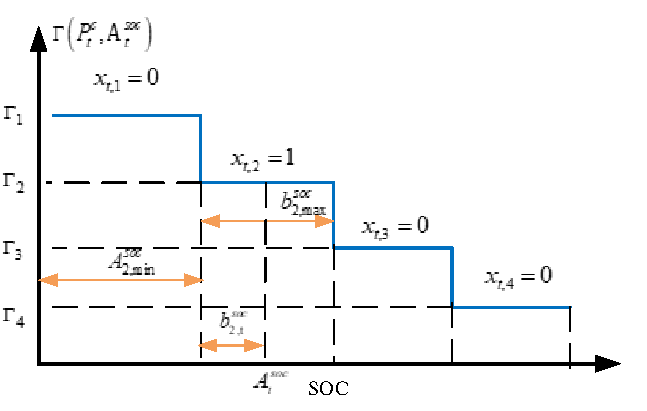
\includegraphics[scale=0.85]{figures/Chap3-3-dual-SOC-approx.pdf}
  \caption{特性曲线$\Gamma \left( {P_t^c,A_t^{soc}} \right)$的近似化处理示例}
  \label{fig:dual-SOC-approx}
\end{figure}

相应地,储气SOC可线性化为,
\begin{subequations}
\label{equ:dual-SOC-approx-example}
\begin{gather}
%m_t^{ch} = P_t^c\sum\nolimits_j {x_{t,j}^{}} {\Gamma _j} \label{equ:non-dual-SOC-approx}\\
A_t^{soc} = \sum\limits_j {({b_{j,t}^{soc} + x_{t,j}^{}A_{j,\min }^{soc}})}, \forall t \label{equ:dual-SOC-approx-example-1} \\
0 \le b_{j,t}^{soc} \le x_{t,j}^{}b_{j,\max }^{soc},\sum\limits_j {x_{t,j}^{}}  = 1, \forall t, j \label{equ:dual-SOC-approx-example-2}
\end{gather}
\end{subequations}
其中,$b_{j,max}^{soc}$表示$A_t^{soc}$的分段$j$的长度;$A_{j,min}^{soc}$表示储气SOC分段$j$的起始值;$b_{j,t}^{soc}$为储气SOC处于分段$j$时偏离 $A_{j,min}^{soc}$的偏移量。(\ref{equ:dual-SOC-approx-example-1})给出了储气SOC的分段线性表示方法;(\ref{equ:dual-SOC-approx-example-2})限制任一分段$j$的偏移量$b_{j,t}^{soc}$不超过该分段的长度。

由于$P_t^cx_{t,j}$项的存在,约束(\ref{equ:non-dual-SOC-approx})为非线性约束,可采用大M法线性化为,
\begin{subequations}
\label{equ:dual-SOC-approx-example-big-M}
\begin{gather}
m_t^{ch} = \sum\limits_j {z_{t,j}}, \forall t \\
P_{\min }^c{x_{t,j}} \le {z_{t,j}} \le P_{\max }^c{x_{t,j}}, \forall t, j\\
P_{\min }^c({1 - {x_{t,j}}})\le {x_{t,j}} - {z_{t,j}} \le P_{\max }^c({1 - {x_{t,j}}}), \forall t,j
\end{gather}
\end{subequations}
其中,$z_{t,j}$为辅助连续量。

AA-CAES储能电站的其它宽工况热力学特性曲线($\Psi$, $\varphi$,$\phi$)亦可采用(\ref{equ:non-dual-SOC-approx})-(\ref{equ:dual-SOC-approx-example-big-M})所示的分段线性化方法进行转化。从而,AA-CAES与风电协同系统调度运行模型转化为混合整数线性规划问题,可通过CPLEX等求解器进行求解。

需要说明的是,采用上述方法近似(\ref{equ:coup-heat-power})及(\ref{equ:coup-mass-SOC})中的热力学特性函数时存在引入了较多整数变量的风险
\footnote{若需减少整数变量个数,可考虑采用文献~\inlinecite{Thesis-Andrew-18}提出的整数变量较少的MILP建模方法。},对模型的求解存在一定影响。考虑到风速的日周期性及日前市场竞标规则,基于滚动优化思想,本节将模型(\ref{eq:WT-CAES-Co-Gen-Model}) 按日分为365个子问题,相邻子问题间通过储气SOC与储热SOC 建立联系,从而实现模型的高效求解。事实上,该类思路在含储能的电力系统运行规划问题中已被采用,如文献~\inlinecite{CXY-Plan-18}。

\subsection{标准风电场算例分析}

本节基于实际风速数据分析风-储协同系统的发电能力,重点关注AA-CAES宽工况运行特性的影响,并进行灵敏度分析,以评估储能容量与储能功率对风-储协同系统发电能力的影响。仿真计算由哈佛大学Odyssey超算服务器集群\footnote{https://www.rc.fas.harvard.edu/odyssey/}与Matlab并行计算工具包完成,模型采用YALMIP\cite{YALMIP}建模,求解器为Gurobi 8.0.1。

\subsubsection{系统参数}
为便于讨论,本节通过将为风电场配置的AA-CAES储能电站的容量分配到单个风机进行分析。选取中国2015年~500~个地区的全年风速数据进行仿真\footnote{风速数据源自 https://www.renewables.ninja/},假定风电场采用金风GW 77/1500系列1.5MW风机,其切入风速为3m/s,额定风速为11m/s, 切出风速为22m/s。

假定与风机协同运行的等效AA-CAES电站采用图\ref{fig:CAES-thermal-struc}所示的两级压缩与两级膨胀结构,压缩机和透平具有相同的额定功率,考虑~1.5MW(Capacity-1)和~1.0MW (Capacity-2)两种情形。除设计质量流率由两种额定功率界定外,其它参数与文献\inlinecite{CAES-IES-16-Rui} 相同,储气库容积为2000m$^3$(1.5MW/12h~储能),工作压力范围为8.4MPa-9MPa。 两级压缩机的设计压比分别为11.5、7.83, 设计等熵效率分别为0.85、0.81,设计入口温度分别为15$^\circ$C、40$^\circ$C。两级透平的设计膨胀比分别为8.94、9.4,设计等熵效率分别为0.82、0.82,设计入口温度均为280$^\circ$C。

%需要说明的是,储气库可采用文献[15]中的钢管储气方案,增设于风机塔筒内部或浅埋于风机附近地下。此外,通过提高储气库的工作压力上限或降低储气库的工作压力下限可降低对储气空间的需求量。

\subsubsection{宽工况影响分析}
配置容量为12h的储能时,所测试的~500~个地区在考虑与不考虑宽工况运行特性时容量因子相对降
低量及不考虑宽工况时的容量因子如图\ref{fig:Part-Load-Exe-Cap}所示。由图\ref{fig:Part-Load-Exe-Cap}可知,对于风资源较贫乏地区,如额定工况下风-储系统的CF低于20\%的区域,计及宽工况后CF的减少量相对较少。其原因在于,该部分地区在实际场景中由于弃风限电等问题并不严重,所配置的储能一般也不进行压缩储能与膨胀释能过程,即实际中无需配置储能。对于风资源较丰富地区,如容量因子大于30\%的区域,AA-CAES宽工况特性对风-储协同运行性能的影响较大,部分地区发电能力下降达5\%。

将所分析的~500~个地区宽工况特性对CF影响的统计特性示于表\ref{tab:Part-load-Wind-CF}。可以得出,对风-储协同系统而言,AA-CAES宽工况运行特性对其发电能力存在不同程度的影响;与不考虑组件部分负载特性相比,考虑宽工况后风资源丰富地区CF降低>4\%。由此可见,宽工况特性对风资源丰富地区的风-储协同系统发电能力的影响不可忽视。
\begin{table}[htb]
  \centering
  \begin{minipage}[t]{0.60\linewidth} % 如果想在表格中使用脚注,minipage是个不错的办法
  \caption{宽工况特性对风-储协同系统CF的影响}
  \label{tab:Part-load-Wind-CF}
    \begin{tabularx}{\linewidth}{ccccc}
      \toprule[1.5pt]
      {\heiti CF 降低百分数} & >4\%  &  >2\% &  >1\%  &   >0.5\%  \\\midrule[1pt]
      Capacity 1 样本数 & 36 & 124 & 179 & 248 \\
      Capacity 2 样本数 & 4 & 102 & 143 & 185 \\
      \bottomrule[1.5pt]
    \end{tabularx}
  \end{minipage}
\end{table}

\begin{figure}[H] % use float package if you want it here
  \centering
  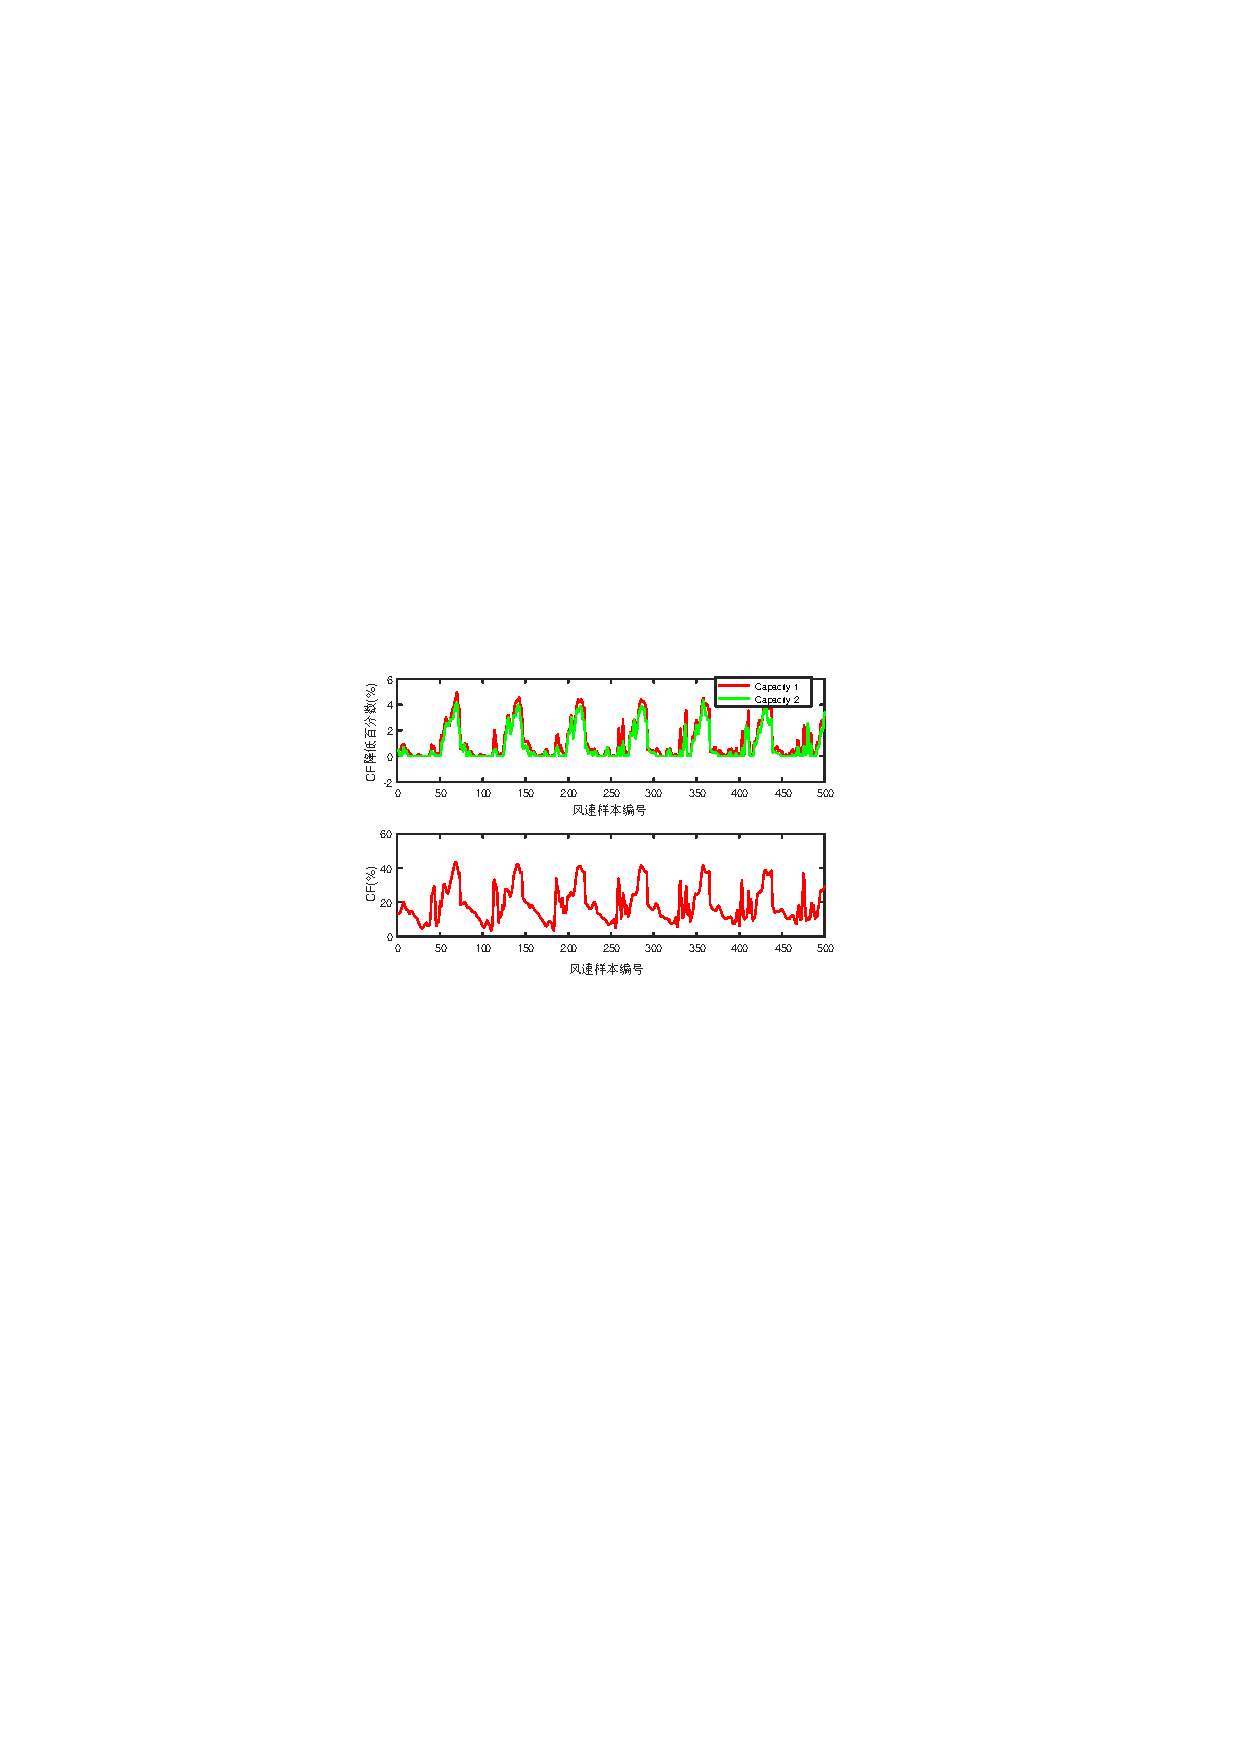
\includegraphics[scale=1.50]{figures/Chap3-15-Part-Load-Exe-Cap.pdf}
  \caption{配置12h储能时宽工况特性对协同系统CF的影响}
  \label{fig:Part-Load-Exe-Cap}
\end{figure}

\subsubsection{灵敏度分析}
对于风资源丰富地区,由于存在较为明显的弃风限电等问题(如图\ref{fig:Wind-Curtailment-Province}所给的典型省份的弃风),一般会配置一定容量的储能,以改善风电与负荷需求的时序不匹配特性。在不同的储能容量下,AA-CAES的宽工况特性对风-储协同系统的影响不同,图\ref{fig:Part-Load-Exe-Str-Sen}给出了不同储能容量时的CF折损的灵敏度分析结果。不难发现,储能容量越大,宽工况特性对风-储协同系统CF的降低(或对500个样本中CF的最大降低量)的影响将会增大,其原因在于在仿真分析中将所有储能容量下的最小储气与储热SOC与设置为最大SOC的5\%;储能容量越大,储进去相同的风电,为了保持最小SOC要求,储能容量大的需要保持较多的能量,才能维持储气罐压力,从而导致其所能释放的风电减少,增大了宽工况对风-储协同运行容量因子的影响。从图~\ref{fig:Part-Load-Exe-Cap}中亦可看出,配置的储能功率越大,宽工况对CF 的影响也越大。因此,在风- 储协同运行场景下,根据风资源情况,实现最佳的AA-CAES容量及功率配置对减小AA-CAES宽工况特性的影响尤为重要。

\begin{figure}[H] % use float package if you want it here
  \centering
  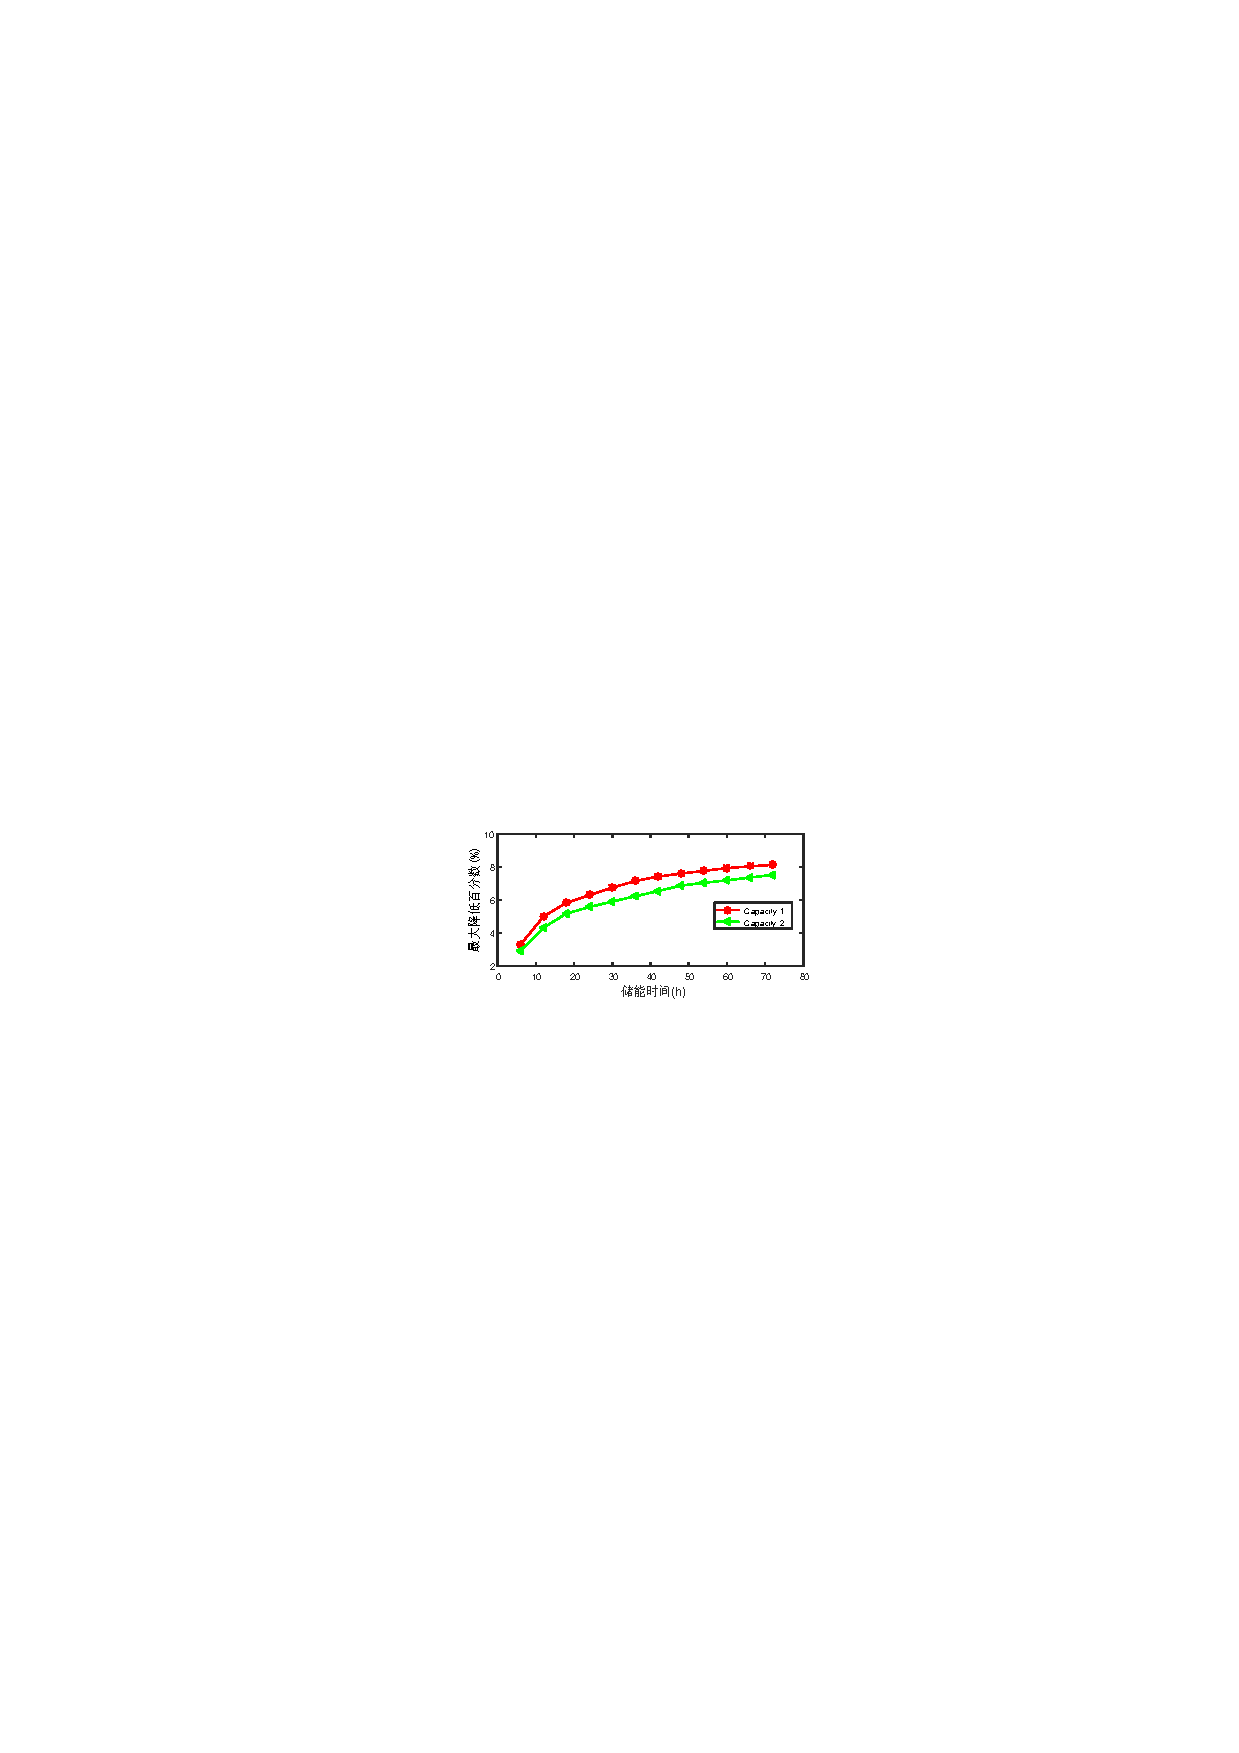
\includegraphics[scale=1.75]{figures/Chap3-15-Part-Load-Exe-Str-Sen.pdf}
  \caption{储能时间对宽工况特性影响程度的灵敏度分析}
  \label{fig:Part-Load-Exe-Str-Sen}
\end{figure}

%\section{含~AA-CAES~储能电站的电网灵活性评估}
%\label{sec:chap3-aa-caes-flex}
%\subsection{面向规划的灵活性评估}
%
%\subsection{模型转化与求解}
%
%\subsection{青海电网算例分析}
%\subsubsection{青海电网概况}
%本文第~\ref{sec:background}节指出了青海电网在可再生能源发展方面的概况。然而,映入眼帘的重要问题是青海100\%清洁能源供给模式可否持续?如何在确保可靠性的条件下实现可持续的100\%清洁能源供应系统?本节通过深入分析青海电网现状、新能源消纳现状,通过“绿电7日”与“绿电9日”模式的分析,挖掘青海电网100\%清洁能源系统不可持续的原因。进一步,基于AA-CAES 能量及备用模型分析储能电站的灵活性,并利用青海电网实际数据\footnote{本节算例中青海电网网架信息由青海电网公司提供,限于部分数据保密要求,该部分数据不予以公开。}合理评估AA-CAES储能电站对于提升可再生能源电力消纳的灵活性。
%
%\subsubsection{结果对比分析}

%\subsubsection{不计及宽工况的双SOC模型}

%\subsubsection{计及宽工况特性的双SOC模型}



%\subsubsection{{ERCOT}电网概况}


%\subsubsection{不计及宽工况的能量及备用模型}

%\subsubsection{计及宽工况的双SOC能量及备用模型}

%\subsubsection{各调度策略综合分析}

\section{面向日前电力市场的储能电站市场运营策略}
\label{sec:chap3-bid-aa-caes}
在储能产业商业化初期,有效的日前电力市场竞标策略可支撑AA–CAES储能电站的经济运行\cite{CAES-DAM-Rui-18}。储能电站参与市场运营的方式主要包括价格影响者机制与价格接受者机制,前者假定储能电站的竞标策略会影响市场电价,后者则在给定的市场价格下决定竞标电量。本节重点研究比较复杂的价格影响者机制下AA-CAES储能电站的竞标策略,并基于此给出价格接受者机制下的竞标策略。首先,在宽工况双SOC能量模型的基础上,提出AA–CAES储能电站的双层竞标策略;其次,在宽工况双SOC能量与备用模型的基础上,给出AA-CAES储能电站以价格接受者参与电量及备用市场的竞标策略。

\subsection{竞标模型}
\label{sec:chap3-bid-aa-caes-game}
本小节研究AA-CAES储能电站以价格影响者机制参与日前电力市场的竞标策略。在价格影响者机制下,一般可采用多层规划来刻画市场参与主体间的交互行为与决策顺序,而多层规划可用主从博弈的思想进行建模与分析\cite{Game-Mei-16}。有鉴于此,我们构建面向AA–CAES电站独立运营商的主从博弈双层竞标模型,以辅助其参与日前电力市场并实现套利运营。主从博弈竞标模型的基本思路为,AA–CAES 储能电站运营商参与电力市场竞标,上报售(购)电量与售(购)电价,以最大化电力交易运营收益;电力市场交易机构根据储能电站、其它电源及负荷的竞标标的,以最大化社会福利出清电力市场。

%其次,提出AA–CAES储能电站主从博弈竞标模型的高效求解方法,其思路为通过最优性条件将该双层非线竞价模型转化为单层模型,并线性化互补松弛约束。 最后,采用布尔展开法近似线性化单层模型目标函数中的价格与电量双线性项,将单层竞价模型转化为混合整数线性规划。

\subsubsection{领导者层:储能电站}
作为市场参与主体,即主从博弈领导者(~Leader~),AA-CAES储能电站运营商以售/购电量与售/购电价为竞标标的,参与日前电力市场竞标以最大化运营收益,
\begin{eqnarray}
\label{equ:aa-caes-pab-leader-obj}
\begin{array}{l}
\mathop {\max \;}\limits_{{\Xi _{UP}}} \sum\limits_{j = 1}^{{N_A}} {\sum\limits_{t = 1}^{{N_T}} {({\lambda _{j,t}^{dis}A_{j,t}^{dis} - \lambda _{j,t}^{ch}A_{j,t}^{ch}})} } - \sum\limits_{j = 1}^{{N_A}} {\sum\limits_{t = 1}^{{N_T}} {({C_j^{dis}A_{j,t}^{dis} + C_j^{ch}A_{j,t}^{ch}})} }
\end{array}
\end{eqnarray}
其中,$N_A$为储能电站运营商所辖的AA-CAES电站个数;$N_T$为日前电力市场总决策时段,本节取为24;$\lambda _{j,t}^{ch}$与$\lambda _{j,t}^{dis}$分别为~AA-CAES~ 储能电站向电力市场的购电报价与售电报价;$A_{j,t}^{ch}$ 与$A_{i,t}^{dis}$ 分别表示电力市场出清的储能电站购电量与充电量,对任一电站$j$,$A_{j,t}^{ch}$与$A_{i,t}^{dis}$ 分别与双SOC模型中的$P_t^c$与$P_t^d$相同\footnote{由于日前电力市场调度时段间隔一般为1h,本节在不引起混淆的情况下混用电量与容量。};$C_j^{ch}$与$C_j^{dis}$分别为电站在压缩储能及膨胀释能模式下的边际运行成本。第一项表示AA-CAES储能电站向电力市场的套利收益(扣除购电成本),第二项表示总的边际运行成本。

AA-CAES储能电站的决策变量$\Xi _{UP}$主要包括向电力市场交易机构上报的竞标标的(售购电量与售购电价),电站自身运行状态量(压缩功率与膨胀功率、储热功率与耗热功率)、储气SOC、 储热SOC等。储能电站主的从博弈竞标策略模型中,上层目标函数的约束条件包括电站自身运行约束与下层模拟的电力市场出清约束,其自身运行约束除包括第\ref{sec:dual-SOC-energy}节提出的双SOC能量模型(\ref{equ:coup-heat-power})、(\ref{equ:coup-mass-SOC})、(\ref{equ:air-SOC-energy})及(\ref{equ:TES-SOC-energy})以及运行限制约束(\ref{eq:WT-CAES-Power-Limit})外,还包括如下的竞标标的限制约束:
\begin{subequations}
\label{equ:aa-caes-pab-bid-cons}
\begin{gather}
0 \le \hat A_{j,t}^{ch} \le u_{j,t}^{ch}\bar A_j^{ch},\;0 \le \hat A_{j,t}^{dis} \le u_{j,t}^{dis}\bar A_j^{dis}, \forall j,t \label{equ:aa-caes-PAB-quantity} \\
\lambda _{j}^{ch,l} \le \lambda _{j,t}^{ch} \le \lambda _{j}^{ch,u},\sum\nolimits_{t = 1}^{{N_T}} {\lambda _{j,t}^{ch}}  \le {N_T}\lambda _{j,av}^{ch} \label{equ:aa-caes-PAB-price-ch},\forall j,t \\
\lambda _{j}^{dis,l} \le \lambda _{j,t}^{dis} \le \lambda _{j}^{dis,u},\sum\nolimits_{t = 1}^{{N_T}} {\lambda _{j,t}^{dis}} \le {N_T}\lambda _{j,av}^{dis} \label{equ:aa-caes-PAB-price-dis}, \forall j,t
\end{gather}
\end{subequations}
其中,$\hat A_{j,t}^{ch}$与$\hat A_{j,t}^{dis}$分别为储能电站售购电量竞标标的;$\bar A_j^{ch}$与$\bar A_j^{dis}$为电站的压缩机容量与膨胀机容量,对于任一电站$j$,其值分别与$P_{max}^c$与$P_{max}^d$相同;$\lambda_j^{ch,l}$(或$\lambda_j^{dis,l}$)与$\lambda_j^{ch,u}$(或$\lambda_j^{dis,u}$)分别为购电电价(或售电电价)的最小值与最大值。(\ref{equ:aa-caes-PAB-quantity})要求向电力市场上报的售购电量竞标标的不能超过其额定压缩与膨胀容量;(\ref{equ:aa-caes-PAB-price-ch})与(\ref{equ:aa-caes-PAB-price-dis})分别限制AA-CAES储能电站的购电电价与售电电价在一定范围内,同时要求平均售/购电价不能超过设定值$\lambda _{j,av}^{dis}$ 与 $\lambda _{j,av}^{ch}$,该值由AA-CAES电站运营商与电力市场签订的合同决定。

\subsubsection{跟随者层:市场出清}
作为AA-CAES储能电站运营商主从博弈竞标策略的跟随者(Follower),电力市场交易机构根据~AA-CAES~储能电站、其它电源及负荷竞标标的,以最大化电力市场社会福利为目标出清电力市场,从而向市场参与主体提供购(售)电量与购(售)电价信号\footnote{此处假定电力市场出清采用以报价结算方式。},即
\begin{eqnarray}
\label{equ:aa-caes-pab-follow-obj}
\begin{array}{l}
\mathop {\min \;}\limits_{{\Xi _{LL}}\;} \sum\limits_{t = 1}^{{N_T}} {\sum\limits_{j = 1}^{{N_A}} {\left[ {\lambda _{j,t}^{dis}A_{j,t}^{dis} - \lambda _{j,t}^{ch}A_{j,t}^{ch}} \right]} } + \sum\limits_{t = 1}^{{N_T}} {\sum\limits_{i = 1}^{{N_G}} {C_{i,t}^gp_{i,t}^g} }  - \sum\limits_{t = 1}^{{N_T}} {\sum\limits_{i = 1}^{{N_D}} {C_{i,t}^dp_{i,t}^d} }
\end{array}
\end{eqnarray}
其中,$C_i^g$ 为常规机组报价;$p_{i,t}^g$为常规机组出清电量;$p_{i,t}^d$ 为负荷出清量;$C_{i,d}$为负荷报价;$N_G$为常规机组个数;$N_D$为负荷个数。目标函数中第一项对应AA-CAES储能电站;第二项与第三项分别对应常规机组与电力负荷。

电力市场出清决策变量${\Xi _{LL}}$主要包括各电源与负荷的中标量、市场出清电价及电网状态变量(线路传输功率、电压等),而约束条件主要包括各电源与负荷运行约束及输电网潮流约束组成。本节采用直流潮流模型描述输电网潮流分布\cite{MATPOWER},具体地:
\begin{subequations}
\label{equ:DC-flow}
\begin{gather}
p_{i,t}^g + W_{i,t}^{} + A_{i,t}^{dis} = A_{i,t}^{ch} + p_{i,t}^d + \sum\limits_{l|F(l) = i} {P_t^l}  - \sum\limits_{l|T(l) = i} {P_t^l} ,\forall i,\forall t \label{equ:DC-flow-bus-power}\\
P_t^l = ({{\theta _{F(l),t}} - {\theta _{T(l),t}}})/{X_l},\forall l,\forall t \label{equ:DC-flow-line-power}\\
0 \le A_{j,t}^{ch} \le \hat A_{j,t}^{ch}, 0 \le A_{j,t}^{dis} \le \hat A_{j,t}^{dis},\;\forall j,\forall t \label{equ:aa-caes-pab-quan-upper}\\
\left\{\begin{aligned}
&0 \le p_{i,t}^g \le p_i^{g,u},0 \le W_{i,t}^{} \le W_{i,t}^u, p_{i,t}^{d,l} \le p_{i,t}^d \le p_{i,t}^{d,u},\;\forall i,\forall t\\
& - P_l^u \le P_t^l \le P_l^u,\forall l,\forall t\\
&  - \pi  \le {\theta _{i,t}} \le \pi ,{\theta _{ref,t}} = 0,\;\forall i,\forall t
\end{aligned}\right.\label{equ:aa-caes-pab-others}
\end{gather}
\end{subequations}
其中,$W_{i,t}$为节点$i$注入的风电功率;$P_t^l$为线路$l$传输的功率;$F(l)$与$T(l)$分别代表线路$l$的首节点与末节点;$\theta _{f(l),t}$ 与$\theta _{t(l),t}$ 表示线路首末节点电压相角;$X_l$为线路阻抗。(\ref{equ:DC-flow-bus-power})描述节点功率平衡关系;(\ref{equ:DC-flow-line-power})描述线路潮流分布;(\ref{equ:aa-caes-pab-quan-upper}) 表征市场出清的AA-CAES储能电站售/购电量(或功率)不超过电站运营商上报的售/购电量(或功率);(\ref{equ:aa-caes-pab-others}) 给定常规机组出力、风电机组出力、线路潮流及节点电压相角的上下限。事实上,由于本节只涉及日前电量市场,因此假定负荷需求全部由日前市场满足,即$ p_{i,t}^{d,l}= p_{i,t}^d = p_{i,t}^{d,u}$,如此目标函数(\ref{equ:aa-caes-pab-follow-obj})中可去除最后一项。

综上,在价格影响者机制下(多个储能电站协同或大容量储能电站情形),AA-CAES电站运营商的主从博弈竞标模型为,
\begin{subequations}
\label{equ:bid-model-price-marker}
\begin{gather}
\mathop {\max \;}\limits_{{\Xi _{UP}}} \sum\limits_{j = 1}^{{N_A}} {\sum\limits_{t = 1}^{{N_T}} {({\lambda _{j,t}^{dis}A_{j,t}^{dis} - \lambda _{j,t}^{ch}A_{j,t}^{ch}})} } - \sum\limits_{j = 1}^{{N_A}} {\sum\limits_{t = 1}^{{N_T}} {({C_j^{dis}A_{j,t}^{dis} + C_j^{ch}A_{j,t}^{ch}})}}\label{equ:bid-model-price-marker-obj}\\
\mbox{s.t.}~
\mbox{AA-CAES双SOC能量模型}\\
\mbox{AA-CAES运行限制约束}\\
\mbox{竞标标的限制约束}\\
\mbox{电力市场出清问题} 
\end{gather}
\end{subequations}

\subsection{竞标模型的典型扩展形式}
\label{sec:chap3-self-schedu}

在第\ref{sec:chap3-bid-aa-caes-game}节中,我们给出了在价格影响者机制下,基于双SOC能量模型的AA-CAES储能电站市场竞标模型。该模型可进一步推广至储能电站容量较小时的价格接受者机制,同时也扩展至计及备用容量及备用调用等情形。本小节重点给出主从博弈竞标模型的几类推广形式,为了表述简洁,此处仅关注单个AA-CAES储能电站,为此相关变量退化采用\ref{sec:dual-SOC}节中的符号。特别地,我们将基于双SOC能量与备用模型给出储能电站以价格接受者同时参与电量及备用市场的竞标模型,以供相应的电力市场运营问题使用。首先,给出不考虑价格不确定性的确定性竞标策略;其次,建立采用盒式不确定集刻画价格不确定性的~AA-CAES~鲁棒竞标策略;最后,给出计及备用调用的随机竞标策略。

\textbf{(1)确定性竞标策略}

当不考虑价格不确定性,采用价格接受者机制时储能电站宽工况竞标模型的目标函数为,
\begin{equation}
\label{equ:aa-caes-self-schedule-DT}
\mathop {\max }\limits_{\Xi_{DT}}  \underbrace {\sum\limits_{t = 1}^{N_T} {\left[ {\lambda_t^E({P_t^d - P_t^c})\Delta t + \lambda_t^{sr}({P_t^{c,sr} - P_t^{d,sr}}) + \lambda_t^{nr}P_t^{d,nr}} \right]} \; - \sum\limits_{t = 1}^{N_T} {({C^{dis}P_t^d + C^{ch}P_t^c})} }_{DT}
\end{equation}
其中,$\lambda_t^E$,$\lambda_t^{sr}$及$\lambda_t^{nr}$分别为日前电量及备用市场中的电量价格、旋转备用与非旋转备用价格。第\ref{sec:chap3-bid-aa-caes-game} 节中我们用$\lambda_t^{dis}$与$\lambda_t^{ch}$区分了价格影响者机制下的膨胀释能与压缩储能过程的竞标电价,此处由于采用了价格接受者机制,用(预测的)市场电价$\lambda_t^E$代替二者。确定性竞标策略的约束集$\Xi_{DT}$由双SOC能量及备用模型(\ref{equ:coup-heat-power})、(\ref{equ:coup-mass-SOC})、(\ref{equ:def-Pc-Pd-eq})、(\ref{equ:air-SOC-reserve})、(\ref{equ:TES-SOC-reserve})、(\ref{equ:coup-mass-heat-SOC-reserve})
以及运行限制约束(\ref{eq:WT-CAES-Power-Limit})界定。

\textbf{(2)鲁棒竞标策略}

若考虑电量价格、旋转备用价格及非旋转备用价格的不确性,可采用不确定性集合来描述电价,进而可构建鲁棒竞标策略。描述不确定性的方式主要有盒式不确定集(无穷范数)、椭球不确定集(欧式范数)以及多面体不确定集(1范数)等\cite{Robust-Self-Schedule-Review-18}。此处仅给出基于盒式不确定集合的竞标策略,若采用其它不确定集描述价格不确定性时,该鲁棒竞标策略亦可相应推广。

盒式不确定集通过无穷范数来约束随机变量,即电量价格、旋转备用及非旋转备用价格可描述为,
\begin{equation}
\label{equ:price-uncertainty-BS}
B{S^\Upsilon } = \left\{ {\tilde \lambda _t^\Upsilon  \in \left[ {\Lambda _t^\Upsilon  - \hat \Lambda _t^\Upsilon ,\;\Lambda _t^\Upsilon  + \hat \Lambda _t^\Upsilon } \right],\left| {\frac{{\tilde \lambda _t^\Upsilon  - \Lambda _t^\Upsilon }}{{\hat \Lambda _t^\Upsilon }}} \right| \le \Psi _B^\Upsilon ,\forall t} \right\},\Upsilon  = \left\{ {E,sr,nr} \right\}
\end{equation}
其中,$\Psi _B^\Upsilon  \in \left[ {0,1} \right],\Upsilon  = \left\{ {E,sr,nr} \right\}$。

基于盒式不确定集的鲁棒竞标目标函数为,
\begin{equation}
\mathop {\max }\limits_\Xi  \mathop {\min }\limits_{\tilde \lambda _t^\Upsilon  \in B{S^\Upsilon }} \left\{ {\sum\limits_{t = 1}^{N_T} {\left[ {\tilde \lambda _t^E({P_t^d - P_t^c}) + \tilde \lambda _t^{sr}({P_t^{c,sr} - P_t^{d,sr}}) + \tilde \lambda _t^{nr}P_t^{d,nr}} \right]} \; - \sum\limits_{t = 1}^{N_T} {({C^{dis}P_t^d + C^{ch}P_t^c})}} \right\}
\end{equation}
从而,基于盒式不确定集的~AA-CAES~鲁棒竞标策略为,
\begin{equation}
\label{equ:aa-caes-self-schedule-BS-uncertainty}
\arg \;\mathop {\max }\limits_\Xi  \left\{ {DT - \Psi _B^E\sum\limits_{t = 1}^{N_T} {\tilde \lambda _t^E({P_t^d - P_t^c})} -\Psi _B^{sr}\sum\limits_{t = 1}^{N_T} {\tilde \lambda _t^{sr}({P_t^{c,sr} - P_t^{d,sr}})} - \Psi _B^{nr}\sum\limits_{t = 1}^{N_T} {\tilde \lambda _t^{nr}P_t^{d,nr}} } \right\}
\end{equation}

%不同于盒式不确定集,椭球不确定集采用欧式范数刻画不确定集\cite{Robust-Self-Schedule-Review-18},即
%\begin{equation}
%\label{equ:price-uncertainty-ES}
%E{S^\Upsilon } = \left\{ {\tilde \pi _t^\Upsilon  \in \left[ {\Pi _t^\Upsilon  - \hat \Pi _t^\Upsilon ,\;\Pi _t^\Upsilon  + \hat \Pi _t^\Upsilon } \right],\sqrt {{{\sum\nolimits_{t = 1}^T {\left( {\frac{{\tilde \pi _t^\Upsilon  - \Pi _t^\Upsilon }}{{\hat \Pi _t^\Upsilon }}} \right)} }^2}}  \le \Psi _E^\Upsilon ,\forall t} \right\},\Upsilon  = \left\{ {E,sr,nr} \right\}
%\end{equation}
%其中,$\Psi _B^\Upsilon  \in \left[ {0,\sqrt {\left| T \right|} } \right],\Upsilon  = \left\{ {E,sr,nr} \right\}$.

%相应地,基于椭球不确定集的~AA-CAES~鲁棒自调度策略为:
%\begin{equation}
%\label{equ:aa-caes-self-schedule-ES-uncertainty}
%\begin{array}{l}
%\arg \;\mathop {\max }\limits_\Omega  \left\{ {DT - \Psi _B^E\sqrt {\sum\limits_{t = 1}^T {{{\left( {\tilde \pi _t^E} \right)}^2}{{\left( {P_t^d - P_t^c} \right)}^2}} }  - \Psi _B^{sr}\sqrt {\sum\limits_{t = 1}^T {{{\left( {\tilde \pi _t^{sr}} \right)}^2}{{\left( {P_t^{c,sr} - P_t^{d,sr}} \right)}^2}} } } \right.\\
%\;\;\;\;\;\;\;\;\;\;\;\;\;\left. { - \Psi _B^{nr}\sqrt {\sum\limits_{t = 1}^T {{{\left( {\tilde \pi _t^{nr}} \right)}^2}{{\left( {P_t^{d,nr}} \right)}^2}} } } \right\}
%\end{array}
%\end{equation}

%(3) 多面体不确定集

%不同于盒式与椭球不确定集,多面体不确定及采用1范数描述不确定集合\cite{Robust-Self-Schedule-Review-18},即电价的鲁棒不确定集为
%\begin{equation}
%\label{equ:price-uncertainty-PS}
%P{S^\Upsilon } = \left\{ {\tilde \pi _t^\Upsilon  \in \left[ {\Pi _t^\Upsilon  - \hat \Pi _t^\Upsilon ,\;\Pi _t^\Upsilon  + \hat \Pi _t^\Upsilon } \right],\sum\nolimits_{t = 1}^T {\left| {\frac{{\tilde \pi _t^\Upsilon  - \Pi _t^\Upsilon }}{{\hat \Pi _t^\Upsilon }}} \right|}  \le \Psi _P^\Upsilon ,\forall t} \right\},\Upsilon  = \left\{ {E,sr,nr} \right\}
%\end{equation}

%由此,基于多面体不确定集的AA-CAES鲁棒自调度策略为:
%\begin{equation}
%\label{equ:aa-caes-self-schedule-PS-uncertainty}
%\begin{array}{l}
%\arg \;\mathop {\max }\limits_\Omega  \left\{ {DT - \Psi _B^E{v^E} - \Psi _B^{sr}{v^{sr}} - \Psi _B^{nr}{v^{nr}}} \right\}\\
%\;\;\;\;\;s.t.\;{v^E} \ge \tilde \pi _t^E\left( {P_t^d - P_t^c} \right),{v^E} \ge 0,\forall t\\
%\;\;\;\;\;\;\;\;\;\;{v^{sr}} \ge \tilde \pi _t^{sr}\left( {P_t^{c,sr} - P_t^{d,sr}} \right),\;{v^{sr}} \ge 0,\forall t\\
%\;\;\;\;\;\;\;\;\;\;{v^{nr}} \ge \tilde \pi _t^{nr}P_t^{d,nr}{v^{nr}} \ge 0,\forall t\;
%\end{array}
%\end{equation}

\textbf{(3)计及备用调用的随机竞标策略}

AA-CAES确定性竞标策略(\ref{equ:aa-caes-self-schedule-DT})及鲁棒竞标策略(\ref{equ:aa-caes-self-schedule-BS-uncertainty})并未考虑实时电力市场中的备用调用,若计及AA-CAES备用容量的调用,即采用双SOC能量及备用扩展模型时,AA-CAES储能电站的宽工况随机竞标模型目标函数为,
\begin{equation}
\label{equ:aa-caes-self-schedule-ST}
\begin{array}{l}
\mathop {\max }\limits_{\Xi_{S}} \sum\limits_{s = 1}^{{N_S}} {{r_s}} \left\{ {\underbrace {\sum\limits_{t = 1}^{N_T} {[ {\lambda _{t,s}^E({P_t^d - P_t^c}) + \lambda _{t,s}^{sr}({P_t^{c,sr} - P_t^{d,sr}}) + \lambda _{t,s}^{nr}P_t^{d,nr}}]} }_{D_{st}^{{R_1}}}} \right.\;\\
\;\;\;\;\;\;\;\; + \underbrace {\sum\limits_{t = 1}^{N_T} {\lambda _{t,s}^E[{({P_t^{d,sr} + P_t^{c,sr}})u_{t,s}^{sr} + P_t^{d,nr}u_{t,s}^{nr}}]} }_{D_{st}^{{R_2}}}\\
\;\;\;\;\;\;\; - \left. {\;\underbrace {\sum\limits_{t = 1}^{N_T} {[{C^{dis}({\overbrace {P_t^d + P_t^{d,sr}u_{t,s}^{sr} + P_t^{d,nr}u_{t,s}^{nr}}^{P_t^{d,Ev}}}) + C^{ch}({\overbrace {P_t^c - P_t^{c,sr}u_{t,s}^{sr}}^{P_t^{c,Ev}}})}]} }_{D_{st}^{{R_3}}}} \right\}
\end{array}
\end{equation}
其中,$r_s$为场景$s$下电力市场电价$\lambda_t^E$,$\lambda_t^{sr}$及$\lambda_t^{nr}$的概率。约束集$\Xi_{S}$由双SOC能量及备用扩展模型(\ref{equ:def-power-relation})、(\ref{equ:air-SOC-reserve-exten})、(\ref{equ:TES-SOC-reserve-exten})、(\ref{equ:coup-heat-power-reserve-exten})以及运行限制约束(\ref{eq:WT-CAES-Power-Limit})共同界定。事实上,模型(\ref{equ:aa-caes-self-schedule-ST})可进一步计及条件风险价值,但不在本章讨论范围之内。

%本文第~\ref{cha:ca-recs} 章会针对风速不确定性讨论基于条件风险价值的新型风-储(压缩空气储能)系统日前电力及备用市场竞标策略。

%\subsection{{ERCOT}算例分析}
%本小节以美国{ERCOT}电网为例,分析AA-CAES储能电站宽工况运行特性对其在电量及备用市场自调度策略的影响,从而明晰在备用特性分析中计及宽工况运行特性的必要性与重要性。此处选择{ERCOT}电网进行分析主要原因在于:1)ERCOT电网电价、负荷及机组参数等公开信息较全面\footnote{国内访问ERCOT电网数据受限,本部分的基础数据由苏黎世联邦理工学院 Jared Garrison 博士提供。};2)ERCOT电网具有很高的风电装机渗透率;3)ERCOT电网具有电量及备用市场;4)ERCOT电网目前规划了D-CAES电站的建设,其规划容量达300MW。需要说明的是,考虑ERCOT电力市场的一种退化情形,即假定电价 具有固定的峰谷价差,即可在一定程度上表征中国电力市场。

\subsection{模型求解策略}
AA-CAES的市场竞标模型及典型各种扩展形式中,以价格影响者机制的主从博弈竞标模型为双层模型,直接求解困难,而其典型扩展形式均为单层模型,比较容易求解。有鉴于此,本小节重点给出双层竞标模型的求解方法,并在下一小节中进行算例分析。

~AA-CAES~电站主从博弈双层竞标模型(\ref{equ:bid-model-price-marker})为非线性模型,下层电力市场出清为线性规划,可利用最优性条件(KKT条件)将该双层模型转化为单层规划。 转化后的单层模型亦为非线性,除AA-CAES热力学特性曲线簇引入的非线性外,其非线性来源主要包括两类,一是通过最优性条件引入的互补松弛约束,二是上层目标函数中价格与能量双线性乘积项。为此,本节采用布尔展开法近似双线性乘积项\cite{Binary-Expansion-1},最终将主从博弈双层竞价模型转化为混合整数线性规划。

\subsubsection{最优性条件}
下层电力市场出清为线性规划, 可采用最优性条件消去其目标函数。 为便于描述,将下层电力市场出清问题(\ref{equ:aa-caes-pab-follow-obj})(\ref{equ:DC-flow})抽象为,
\begin{eqnarray}
\begin{array}{l}
\min \;{f^T}x\\
s.t.\;\;{A_{eq}}x = {b_{eq}}:\;\lambda \\
\;\;\;\;\;\;{A_{ineq}}x \le {b_{ineq}}:\mu
\end{array}
\end{eqnarray}
其对应的等价~KKT~系统为,
\begin{subequations}
\label{eq:EKKT}
\begin{gather}
{A_{eq}}x = {b_{eq}}, {A_{ineq}}x \le {b_{ineq}}, f = A_{eq}^T\lambda  - A_{ineq}^T\mu, \\
 0 \le {\mu} \bot ({ - {A_{ineq}}x + {b_{ineq}}}) \ge 0 \label{eq:KKT-non}
\end{gather}
\end{subequations}

最优性条件(\ref{eq:EKKT})中引入了非线性互补松弛约束(\ref{eq:KKT-non}),其抽象形式为,
\begin{eqnarray}
\label{eq:add}
0 \le \left( {a - f} \right) \bot g \ge 0
\end{eqnarray}
为便于求解,将(\ref{eq:add})线性化为
\begin{eqnarray}
\label{equ:aa-caes-big-M}
0 \le a - f \le Mh,\;0\le g \le M\left( {1 - h} \right)
\end{eqnarray}
其中,$h$为引入的布尔量;$M$ 为一足够大的正数。

\subsubsection{布尔展开法}
上层目标函数(\ref{equ:aa-caes-pab-leader-obj})中存在电价与电量相乘的双线性项,如$\lambda _{j,t}^{dis}A_{j,t}^{dis}$与$\lambda _{j,t}^{ch}A_{j,t}^{ch}$。 针对该类双线性项,采用布尔展开法\cite{Binary-Expansion-1,Binary-Expansion-2}近似线性化。以线性化$\lambda _{j,t}^{dis}A_{j,t}^{dis}$为例,可将$\lambda _{j,t}^{dis}$展开为,
\begin{eqnarray}
\label{equ:aa-caes-ben-1}
\lambda _{j,t}^{dis} = \lambda _j^{dis,l} + \Delta \lambda _j^{dis}\sum\limits_{k = 0}^{{K_1}} {{2^k}} x_{j,t,k}^{dis},\forall j,\forall t
\end{eqnarray}
并附加如下约束,
\begin{subequations}
\label{equ:aa-caes-ben-append}
\begin{gather}
0 \le A_{j,t}^{dis} - z_{j,t,k}^{dis} \le M({1 - x_{j,t,k}^{dis}}),\forall j,\forall t,\forall k\\
0 \le z_{j,t,k}^{dis} \le Mx_{j,t,k}^{dis},\forall j,\forall t,\forall k\\
\Delta \lambda _j^{dis} = ({\lambda _j^{dis,u} - \lambda _j^{dis,l}})/G,\;G = {2^{{K_1}}},\forall j
\end{gather}
\end{subequations}
其中,$x_{j,t,k}^{dis}$为引入的辅助布尔变量;$z_{j,t,k}^{dis}$为辅助连续量;$\Delta \lambda _j^{dis}$为售电电价的离散步进量。$\lambda _{j,t}^{ch}A_{j,t}^{ch}$ 亦可采用相同的方式线性化。

布尔展开式(\ref{equ:aa-caes-ben-append})的近似精确度可通过离散点个数进行控制,引入的布尔量与离散点数的复杂度为[$O(\log_2{K})$],其中~$K$~为近似段数。例如,对于区间[0,1] 的连续量采用32个离散点近似时,只需5个布尔量即可。此外,AA-CAES双SOC模型中的特性曲线的近似处理可采用第
\ref{sec:wind-ESS-operation-model-appro}中的转化方法。

经过上述变换,面向日前电力市场的~AA-CAES~储能电站主从博弈竞标模型的MILP近似模型的目标函数为,
\begin{eqnarray}
\begin{array}{l}
\mathop {\max \;}\limits_{\Xi_{UP-MILP}} \sum\limits_{t = 1}^{{N_T}} {\sum\limits_{j = 1}^{{N_A}} {[{\lambda _j^{dis,l}A_{j,t}^{dis} + \Delta \lambda _j^{dis}\sum\limits_{k = 0}^{{K_1}} {{2^k}} z_{j,t,k}^{dis}}]} } \\
\;\;\;\;\;\;\;\;\; - \sum\limits_{t = 1}^{{N_T}} {\sum\limits_{j = 1}^{{N_A}} {[{\lambda _j^{ch,l}A_{j,t}^{ch} + \Delta \lambda _j^{ch}\sum\limits_{k = 0}^{{K_2}} {{2^k}} z_{j,t,k}^{ch}}]} } \\
\;\;\;\;\;\;\;\;\; - \sum\limits_{j = 1}^{{N_A}} {\sum\limits_{t = 1}^{{N_T}} {[{C_j^{dis}A_{j,t}^{dis} - C_j^{ch}A_{j,t}^{ch}}]} }
\end{array}
\end{eqnarray}
其中,可行域$\Xi_{UP-MILP}$由以下约束限定:宽工况双SOC运行约束及其近似化方法,电站电量及电价竞标标的约束(\ref{equ:aa-caes-pab-bid-cons}),电力市场出清条件~KKT~系统中的等式约束(\ref{eq:EKKT}),采用大~M~法线性化非线性互补约束~(\ref{eq:KKT-non})~ 后得到的线性约束(\ref{equ:aa-caes-big-M}),线性化目标函数引入的约束(\ref{equ:aa-caes-ben-1})-(\ref{equ:aa-caes-ben-append}),以及采用(\ref{equ:dual-SOC-approx-example}) 与(\ref{equ:dual-SOC-approx-example-big-M})的方法近似的热力学特性曲线簇。

\subsection{IEEE系统算例分析}
本小节采用改进的~IEEE-24~节点可靠性测试系统分析AA-CAES储能电站的主从博弈竞标策略。该测试系统拓扑可参见文献\inlinecite{CAES-DAM-Rui-18},主要包含10台发电机组、32条输电线路、6座风电场、1座AA-CAES电站。AA-CAES电站布置于母线\#19,风电场位于母线 \#3,\#5,\#7,\#16,\#21,\#23。AA-CAES电站采用两级压缩、两级膨胀结构,采用常压-滑压运行方式,具体参数如表\ref{tab:AA-CAES-para}所示,其它机组参数、线路参数可参考文献\inlinecite{IEEE-RTS-24-2016}。%~AA-CAES~ 电站内部热力学特性曲线采用第~\ref{sec:chap2-bound-measure}节仿真参数。

\begin{table}[htb]
  \centering
  \begin{minipage}[t]{0.65\linewidth} % 如果想在表格中使用脚注,minipage是个不错的办法
  \caption{AA-CAES储能电站参数}
  \label{tab:AA-CAES-para}
    \begin{tabularx}{\linewidth}{ccccc}
      \toprule[1.5pt]
    参数 & $\bar A^{\rm ch}$,$\bar A^{\rm dis}$ & $\lambda^{\rm ch}$,$\lambda^{\rm dis}$ & $pr$ & $\lambda_{\rm av}^{\rm ch}$,$\lambda_{\rm av}^{\rm dis}$ \\\midrule[1pt]
  单位 & MW & $\$$/MWh & MPa & $\$/$MWh \\
  数值 & 150,350 & [35.55,69.47] & [8.4,9.0]&  47.47 \\
      \bottomrule[1.5pt]
    \end{tabularx}
  \end{minipage}
\end{table}

%\subsubsection{等效电池模型结果}
%\subsubsection{双SOC模型结果}
%\subsubsection{讨论与分析}

系统中各电源在各时段的报价最大值、最小值及平均值如图\ref{fig:AA-CAES-PAB-Price}所示,假定AA-CAES储能电站压缩储能电价与膨胀释能电价在各电源报价的最大与最小值之间。同时,储能电站24 时段平均报价不能超过各电源边际电价确定的平均值。

\begin{figure}[H] % use float package if you want it here
  \centering
  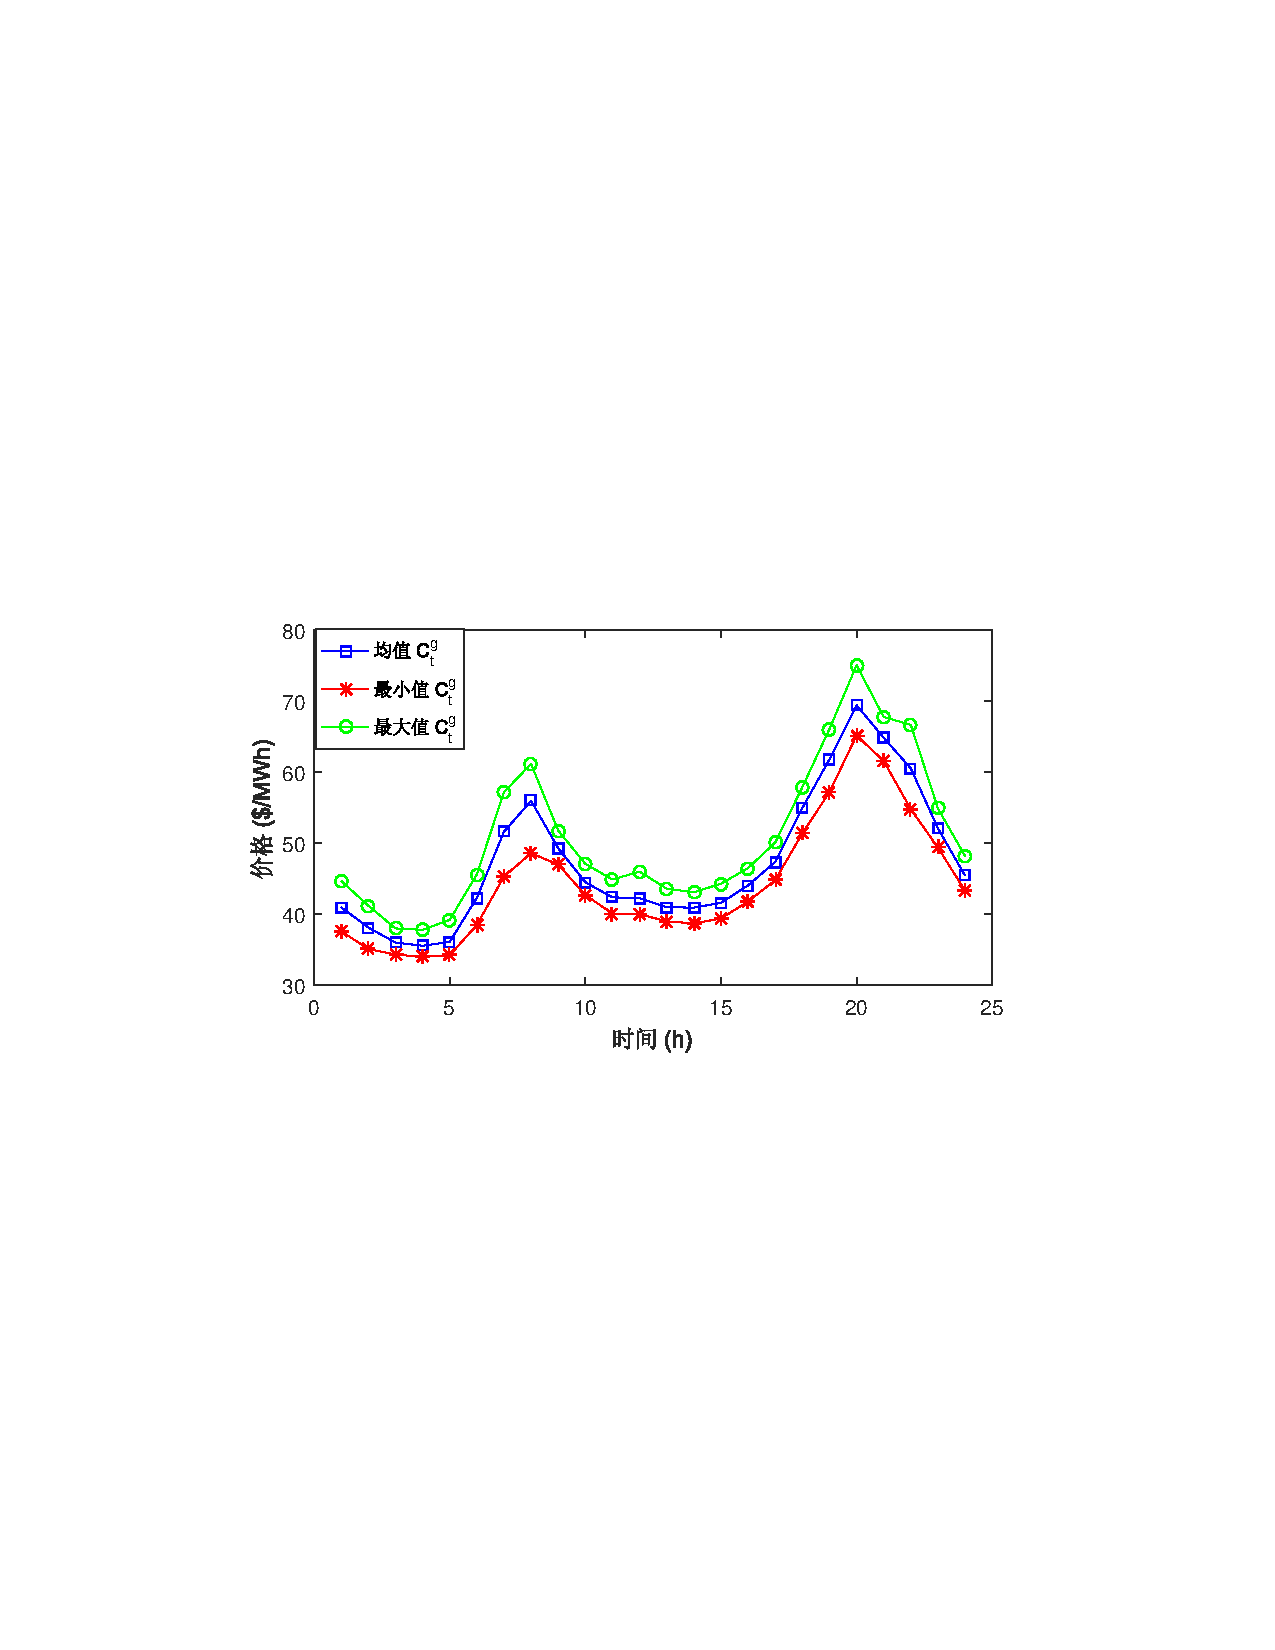
\includegraphics[scale=0.72]{figures/Chap3-10-PAB-Price.pdf}
  \caption{常规机组边际电价}
  \label{fig:AA-CAES-PAB-Price}
\end{figure}

图\ref{fig:Part-Load-PAB-Bid}给出了AA--CAES日前电力市场主从博弈竞标策略,包含购/售电价标的与购/售电量标的,图~\ref{fig:AA-CAES-PAB-LoadGen}给出了系统各电源出力水平。 AA-CAES储能电站在时段6至时段9时压缩储能,并在系统负荷高峰期其它电源难以满足系统总负荷需求时以高价释能售电,如时段11、12、15、16、19、20 等。

\begin{figure}[H] % use float package if you want it here
  \centering
  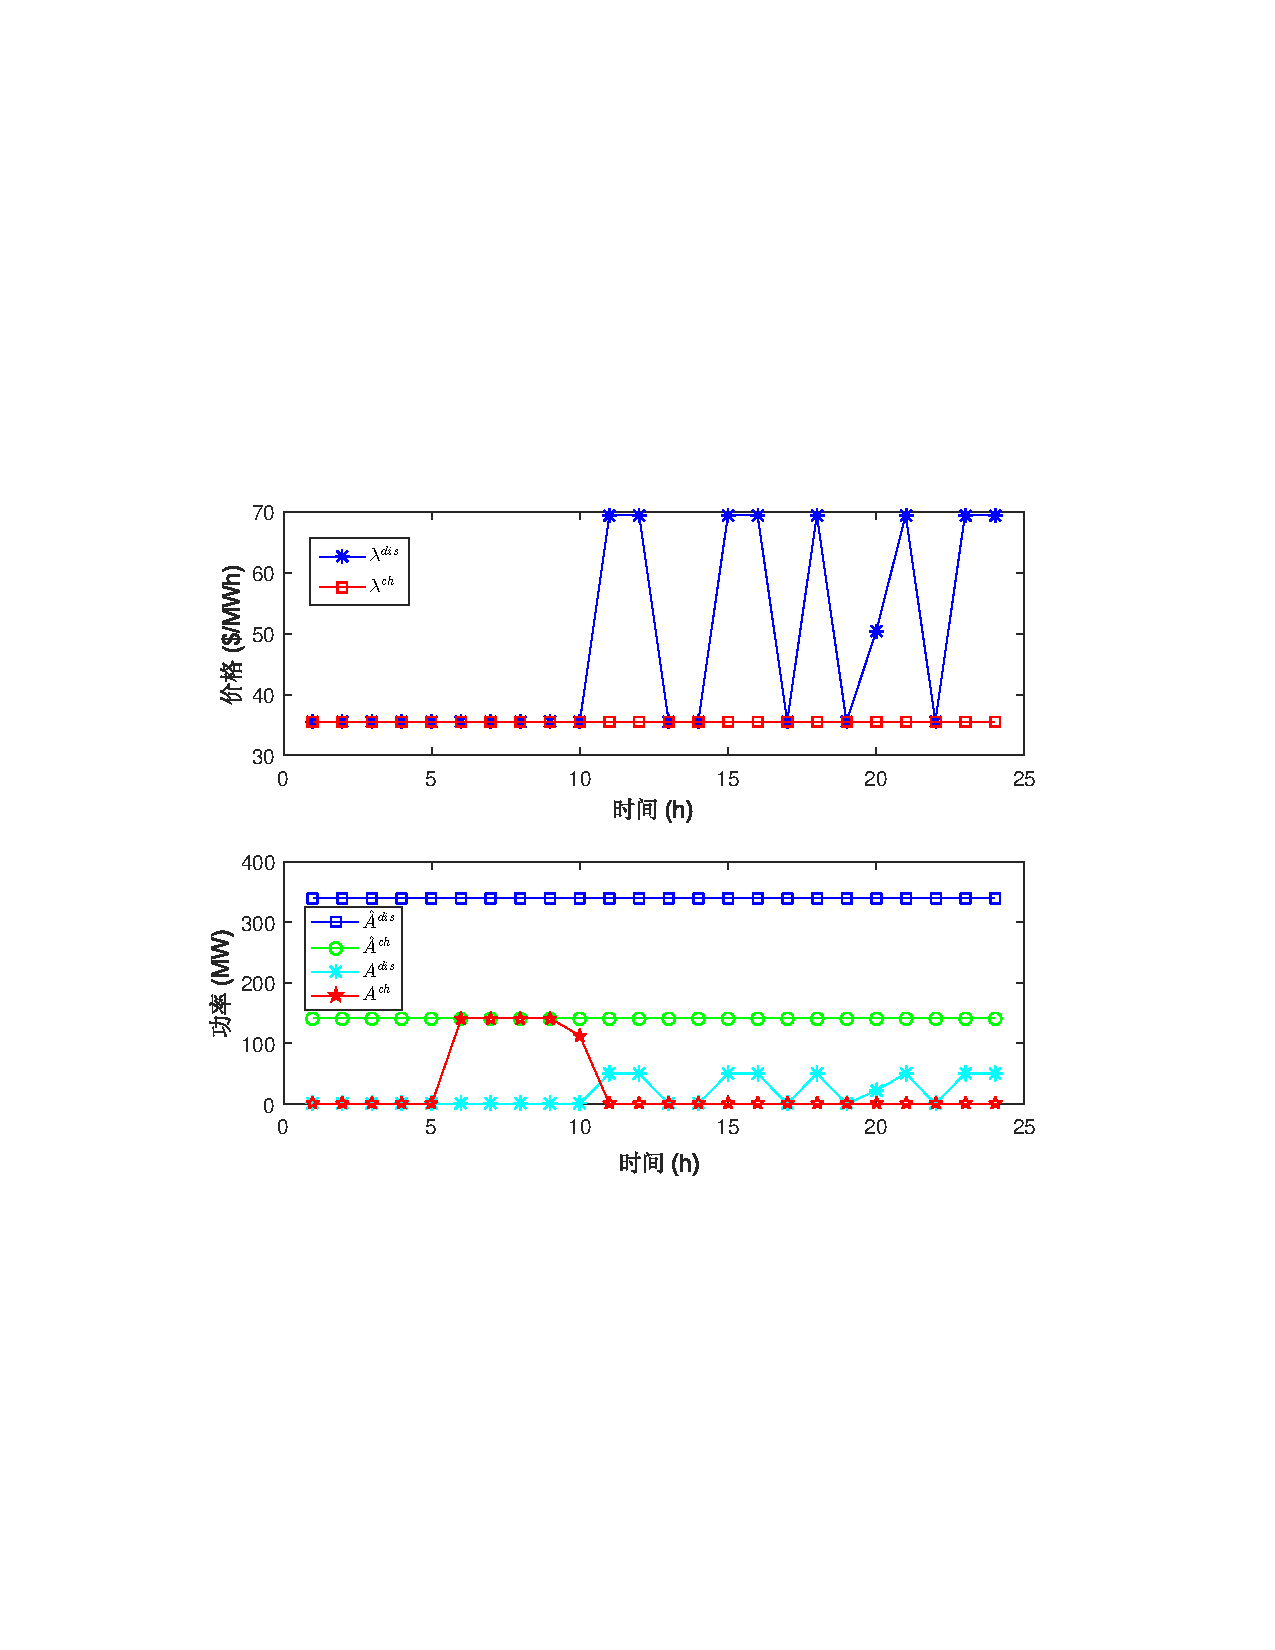
\includegraphics[scale=0.70]{figures/Chap3-10-PAB-Bid.pdf}
  \caption{AA-CAES储能电站竞标策略}
  \label{fig:Part-Load-PAB-Bid}
\end{figure}

由图\ref{fig:AA-CAES-PAB-Price}与图\ref{fig:Part-Load-PAB-Bid} 可知,AA-CAES电站以低价购入电量,再以高价售出电量,从而实现套利运营,在当前策略下日前套利运营的收益为\$19548。 特别地, 由于本节市场机制采用按报价支付的方式结算,AA-CAES~电站运营商以最高价 \$69.47 作为售出电价报价,以最低价\$35.55 作为购入电价报价,同时为满足报价平均值限制,部分时刻如时段20以低于最高价的价格报价。

\begin{figure}[H] % use float package if you want it here
  \centering
  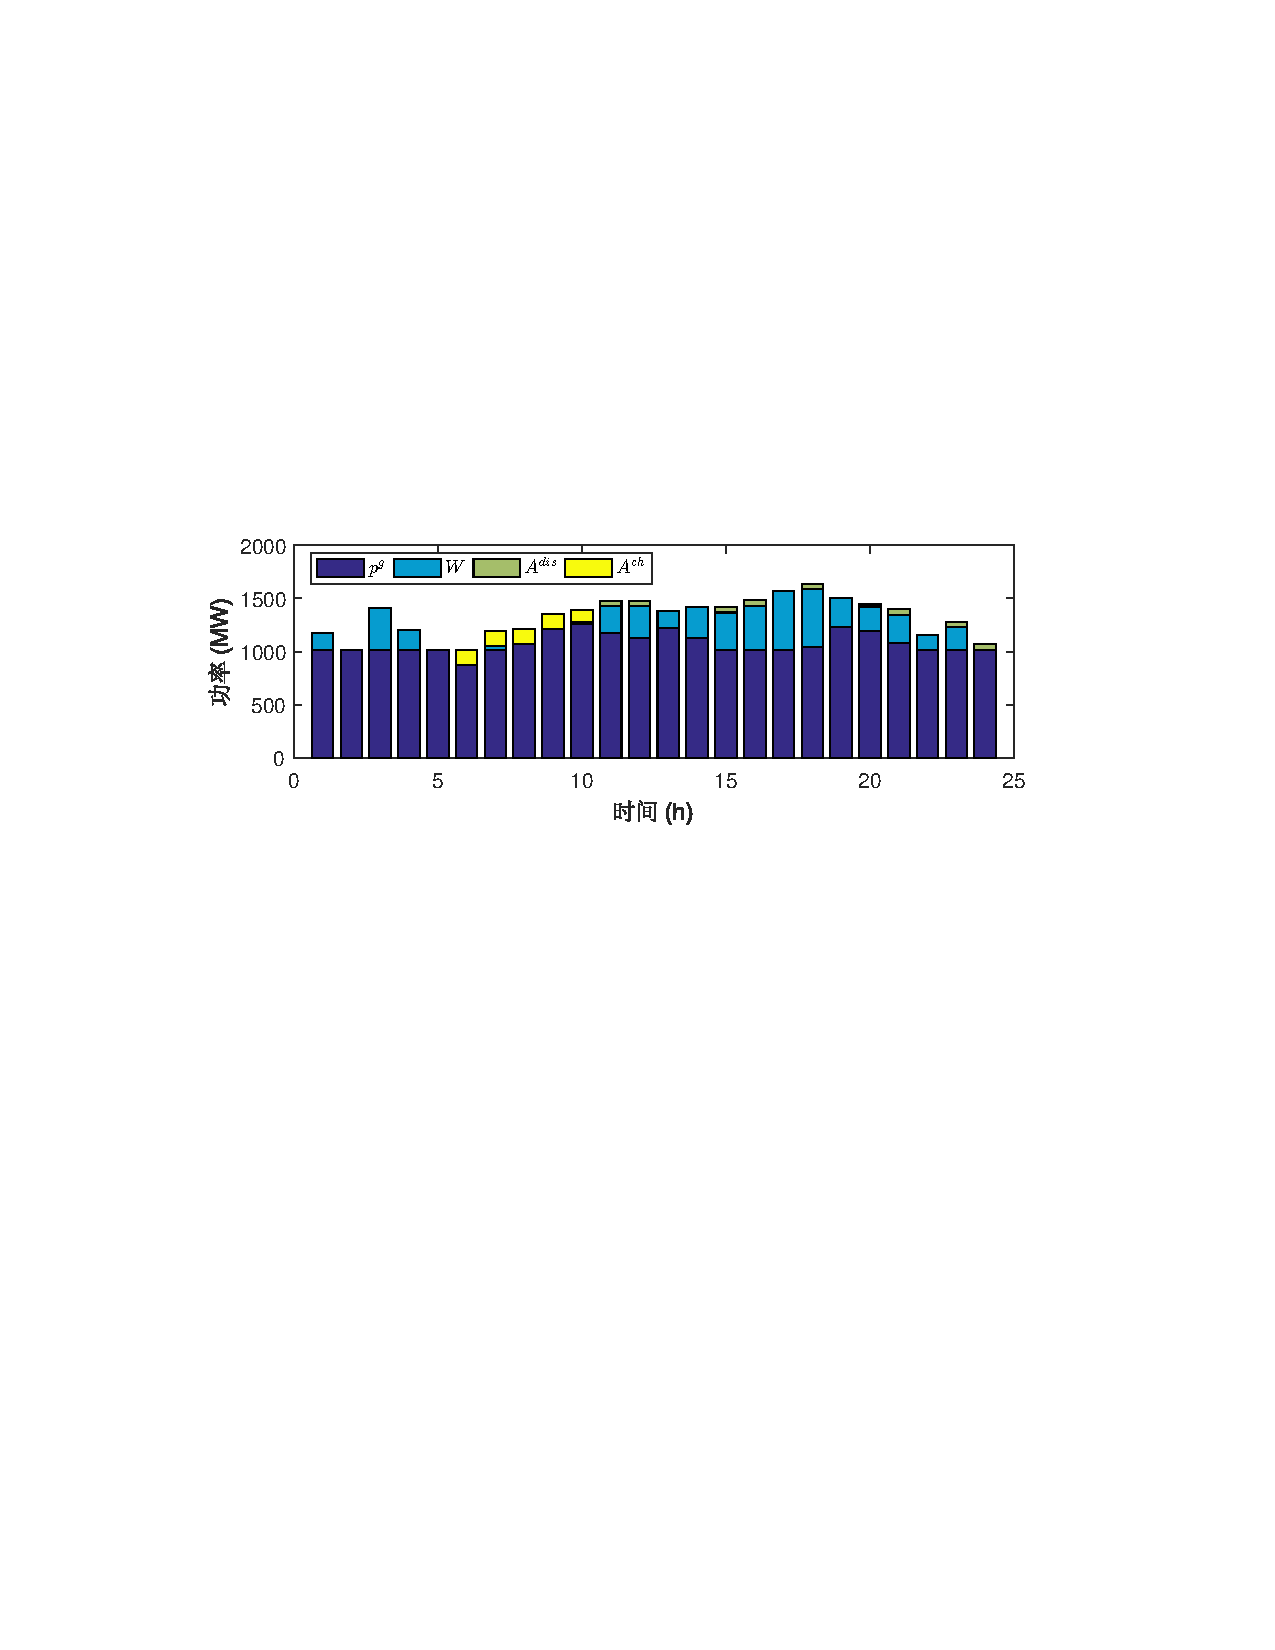
\includegraphics[scale=0.75]{figures/Chap3-10-PAB-LoadGen.pdf}
  \caption{系统各电源出力水平}
  \label{fig:AA-CAES-PAB-LoadGen}
\end{figure}

\begin{figure}[H] % use float package if you want it here
  \centering
  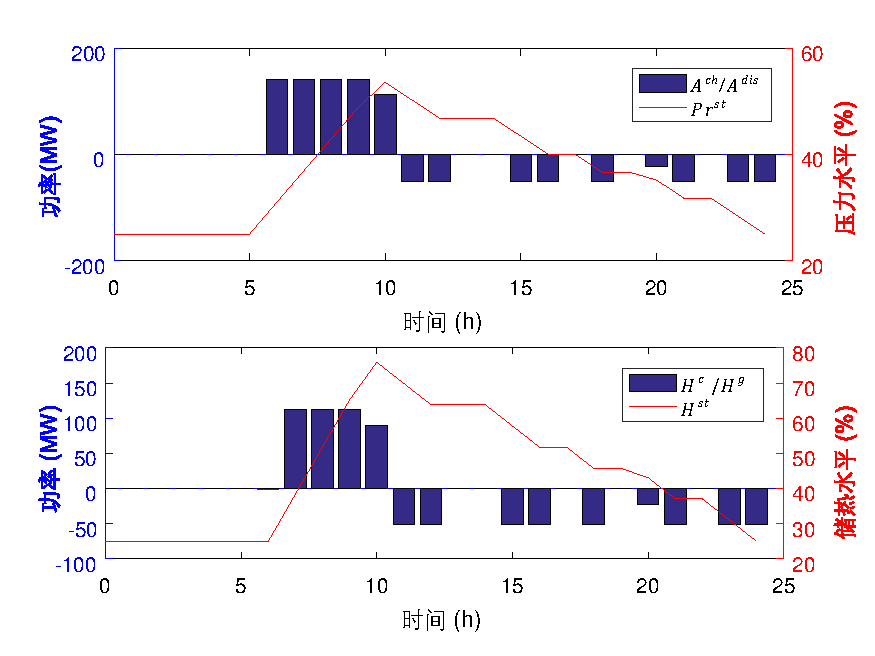
\includegraphics[scale=0.75]{figures/Chap3-10-PAB-SOC.pdf}
  \caption{AA-CAES储气水平和储热水平变化情况}
  \label{fig:Part-Load-PAB-SOC}
\end{figure}

图~\ref{fig:Part-Load-PAB-SOC}~给出了~AA-CAES~储能电站内部储气罐压力变化情况与储热水平变化情况。系统初始储热水平及储气库储气水平(百分比)均为25\%,AA-CAES压缩储能过程中储气水平增加,收集压缩热能提升储热水平。~AA-CAES~电站膨胀释能过程中储气室储气水平下降,由于透平发电环节需要回馈压缩热能,从而使得储热水平下降。储热系统中富余的压缩热能可供集中供暖,从而有望进一步提升~AA-CAES~电站运行收益,第4章将对此进行深入分析。图中亦可得知,压缩储能阶段几乎以额定工况运行,部分负载特性的影响不显著,膨胀释能常以部分负载工况运行,存在潜在备用收益,备用收益与部分负载导致的低效运行之间的平衡尚需进一步研究。

\section{小结}
AA-CAES技术方案最为直接的应用形式为储能电站,然而不同于常规电池储能等,AA-CAES储能电站内部具有独特的压力势能与压缩热能的解耦存储与耦合释能特性。同时,在电力系统外界宽工况运行要求下,AA-CAES储能电站的内部组件具有明显的部分负载特性。本章借鉴电池储能建模中的SOC方法,提出了基于热力学特性曲线簇的AA-CAES宽工况双SOC能量模型,能量与备用模型及扩展形式,进一步研究了计及宽工况特性的AA-CAES储能电站调度策略及日前电力市场竞标策略,为以储能电站形式应用于电力系统的AA-CAES的建模、运行及运营等问题提供了初步的建模方法。
